%%\documentclass[sigconf]{acmart}
\documentclass[sigconf]{acmart}
\usepackage{subcaption}
\usepackage[ruled,vlined,linesnumbered]{algorithm2e}
\usepackage{multirow}
\usepackage{makecell}

\SetAlFnt{\small}  
\SetAlCapNameFnt{\small} 

\SetCommentSty{blue}

\SetCommentSty{mybluecomment}
\newcommand{\mybluecomment}[1]{\textcolor{blue}{#1}}

\SetKwBlock{Critical}{begin critical}{end}

\setlength{\textfloatsep}{6pt}
\setlength{\floatsep}{6pt}
\setlength{\intextsep}{6pt}

\setlength{\abovecaptionskip}{4pt}
\setlength{\belowcaptionskip}{0pt}

\AtBeginDocument{%
  \providecommand\BibTeX{{%
    Bib\TeX}}}

%  The following info Sandeep placed from email he got. If you think something is wrong, please dont edit. Inform sandeep, please. 
\copyrightyear{2026}
\acmYear{2026}
\setcopyright{cc}
\setcctype{by}
\acmConference[ICPP '26]{Proceedings of the 55th International Conference on Parallel Processing}{September 28-October 01, 2026}{Singapore, Singapore}
\acmBooktitle{Proceedings of the 55th International Conference on Parallel Processing (ICPP '26), September 28-October 01, 2026, Singapore, Singapore}
\acmDOI{10.1145/3832810.3832887}
\acmISBN{979-8-4007-2657-6/2026/09}

\newcommand{\REM}[1]{}


\begin{document}

\title{BP-MDS: Million-Scale Approximate CVRP in Minutes via Parallel Divide-and-Conquer}
% Snadeep: Adding state, as got some warnings while submitting to TAPS

\author{Chekkala Sandeep Reddy}
\orcid{0009-0001-1398-7436}
\authornote{Corresponding author}
\affiliation{%
  \institution{Indian Institute of Technology Madras}
  \city{Chennai}
  \country{India}}
\email{sandeep.chekkala.wh@gmail.com}

\author{Lakshya Rani P}
\orcid{0009-0008-0157-0941}
\affiliation{%
  \institution{Indian Institute of Technology Madras}
  \city{Chennai}
  \country{India}}
\email{cs22b047@smail.iitm.ac.in}

\author{Somesh Singh}
\orcid{0000-0002-7648-9979}
\affiliation{%
  \institution{Siemens EDA} 
  \city{Meylan} 
  \country{France} 
}
\email{somesh.singh@siemens.com} 

\author{Rajesh Pandian Muniasamy}
\orcid{0000-0003-4702-4678}
\affiliation{%
  \institution{Qualcomm}
  \city{Bangalore}
  \country{India}}
\email{mrpraj@gmail.com}

\author{Rupesh Nasre}
\orcid{0000-0001-7490-625X}
\authornote{Partially supported by the FedEx Centre research grant SB24250339CSFEDX008103}
\affiliation{%
  \institution{Indian Institute of Technology Madras}
  \city{Chennai}
  \country{India}}
\email{rupesh@cse.iitm.ac.in}


\begin{abstract}
The Capacitated Vehicle Routing Problem (CVRP) is a well-known NP-hard problem with wide applications in logistics and transportation.  Given the combinatorial nature of the problem, a diverse set of heuristics has been proposed in the literature to obtain approximate solutions to CVRP. Prior research has largely focused on small- and medium-sized instances, having up to a few thousand customers. With growing instance sizes and problem complexity in logistics and transportation, there is a pressing need to design scalable techniques for CVRP. The current state-of-the-art CVRP heuristics struggle to scale to large problem instances, taking prohibitively long to arrive at a reasonable solution and also having a massive memory footprint. We introduce BP-MDS, a parallel divide-and-conquer framework for approximate CVRP that targets large-scale (million-customer) instances while achieving low optimality gaps. BP-MDS decomposes the problem into smaller subproblems that are processed concurrently, exhibiting empirically near-linear scalability with respect to input size and strong scaling across threads. Experimental results show that BP-MDS achieves $20\times$--$60\times$ speedups over ParMDS and up to $100\times$ (single-threaded) and $2370\times$ (multi-threaded) speedups over HGS-CVRP. BP-MDS solves CVRP instances with up to 5 million customers in 8 minutes.
\end{abstract} 

%%
%% The code below is generated by the tool at http://dl.acm.org/ccs.cfm.
%% Please copy and paste the code instead of the example below.
%%

%%
%% CCS Concepts tuned for ICPP 2026
%% Verified via https://dl.acm.org/ccs
%%

\begin{CCSXML}
<ccs2012>
   <concept>
       <concept_id>10010520.10010521.10010528.10010536</concept_id>
       <concept_desc>Computer systems organization~Multicore architectures</concept_desc>
       <concept_significance>500</concept_significance>
       </concept>
   <concept>
       <concept_id>10003752.10003809.10011254.10011257</concept_id>
       <concept_desc>Theory of computation~Divide and conquer</concept_desc>
       <concept_significance>500</concept_significance>
       </concept>
   <concept>
       <concept_id>10003752.10003809.10003635</concept_id>
       <concept_desc>Theory of computation~Graph algorithms analysis</concept_desc>
       <concept_significance>300</concept_significance>
       </concept>
   <concept>
       <concept_id>10010147.10010169.10010170</concept_id>
       <concept_desc>Computing methodologies~Parallel algorithms</concept_desc>
       <concept_significance>300</concept_significance>
       </concept>
 </ccs2012>
\end{CCSXML}

\ccsdesc[500]{Computer systems organization~Multicore architectures}
\ccsdesc[500]{Theory of computation~Divide and conquer}
\ccsdesc[300]{Theory of computation~Graph algorithms analysis}
\ccsdesc[300]{Computing methodologies~Parallel algorithms}


%%
%% Keywords tuned for ICPP 2026
%%
\keywords{Capacitated Vehicle Routing Problem (CVRP), Parallel Divide-and-Conquer, OpenMP, Large-Scale Optimization, High Performance Computing (HPC), Approximation Algorithms}
\maketitle


\section{Introduction}
\label{sec::introduction}


\begin{figure*}[htbp]
    \centering
    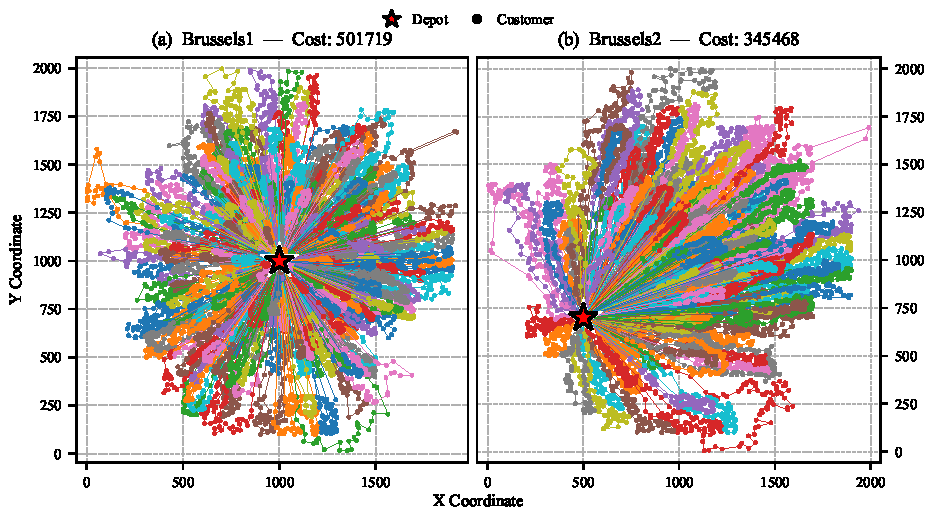
\includegraphics[width=\textwidth, height=0.4\textheight]{assets/BKS_Brussels1_Brussels2_combined.pdf}
    \caption{Best Known Solution (BKS) for Brussels instances from CVRPLIB~\cite{CVRPLIB}, exhibiting a flower-like routing pattern}
    \label{fig:BKS_Brussels}
\end{figure*}

%The Capacitated Vehicle Routing Problem (CVRP) is a fundamental combinatorial optimization problem in which a fleet of vehicles with limited capacity must serve a set of customers with known demands, starting and ending at a central depot, while minimizing the total routing cost.

The Capacitated Vehicle Routing Problem (CVRP) is a fundamental combinatorial optimization problem. 
It involves a fleet of vehicles with limited capacity that serve a set of customers with known demands, starting and ending at a central depot, while minimizing the total distance traveled. Algorithms developed for CVRP are widely applicable to transportation and delivery optimization problems. Several variants of CVRP have been studied, including environmentally aware formulations that minimize carbon emissions \cite{Bektas_Laporte_PRP} and variants with customer time window constraints \cite{Solomon_VRPTW}. The NP-hard nature of the problem renders exact approaches impractical for large instances, motivating the use of approximation algorithms and heuristic methods. Due to the practical importance and theoretical challenge posed by CVRP, it has received significant attention in the literature~\cite{pecin2017new, arnold2019efficiently}. Unfortunately, most of these studies are limited to relatively smaller instances. The approximation algorithms and heuristics primarily target instances with only a few hundred to a few thousand customers. In the logistics sector, while small and medium instance sizes permit optimizing for local warehouses, optimizing across multiple cities and countries necessitates a global consideration involving millions of customers. However, theoretical bounds and practical limitations prevent the existing efficient methods from scaling.

Our goal in this work is to design a solver for million-scale CVRP. In particular, we propose finding a solution to large CVRP instances within minutes without adversely affecting the solution quality. Our method utilizes a new parallel divide-and-conquer algorithm to decompose the geometry into smaller instances, to solve them concurrently via a minimum spanning tree construction, and to escape the local extrema via randomization. The main contributions of this paper are as follows.

1) \textbf{Parallel Divide-and-Conquer Framework with Strong Scalability}: 
We propose a spatial decomposition-based approach that first partitions the problem into independent subproblems, followed by MST-guided route construction within each partition and randomized DFS-based exploration. The method exhibits strong scalability with respect to both problem size (up to million-scale instances) and parallel execution on multi-core architectures.

2) \textbf{Open-Source Parallel Implementation}\footnote{Publicly available source code: \url{https://github.com/CodeCraftsmanSandeep/BP-MDS}}: We provide an optimized OpenMP-based parallel CPU implementation, called BP-MDS, which incorporates efficient load balancing, on-demand memory allocation, and a customized min-heap design that avoids constructing the complete graph, resulting in significant reductions in CVRP execution time and memory consumption.

3) \textbf{Thorough Experimental Evaluation}: 
We demonstrate that our algorithm efficiently solves million-scale CVRP instances, handling inputs of up to 5 million nodes within 8 minutes. Across standard benchmark datasets, BP-MDS achieves an overall geometric mean optimality gap of 8.51\% 
(9.67\% on CVRPLIB~\cite{CVRPLIB} (130 instances) and 1.27\% on FILO2~\cite{FILO2} (20 instances)).



\begin{figure*}[htbp]
    \centering
    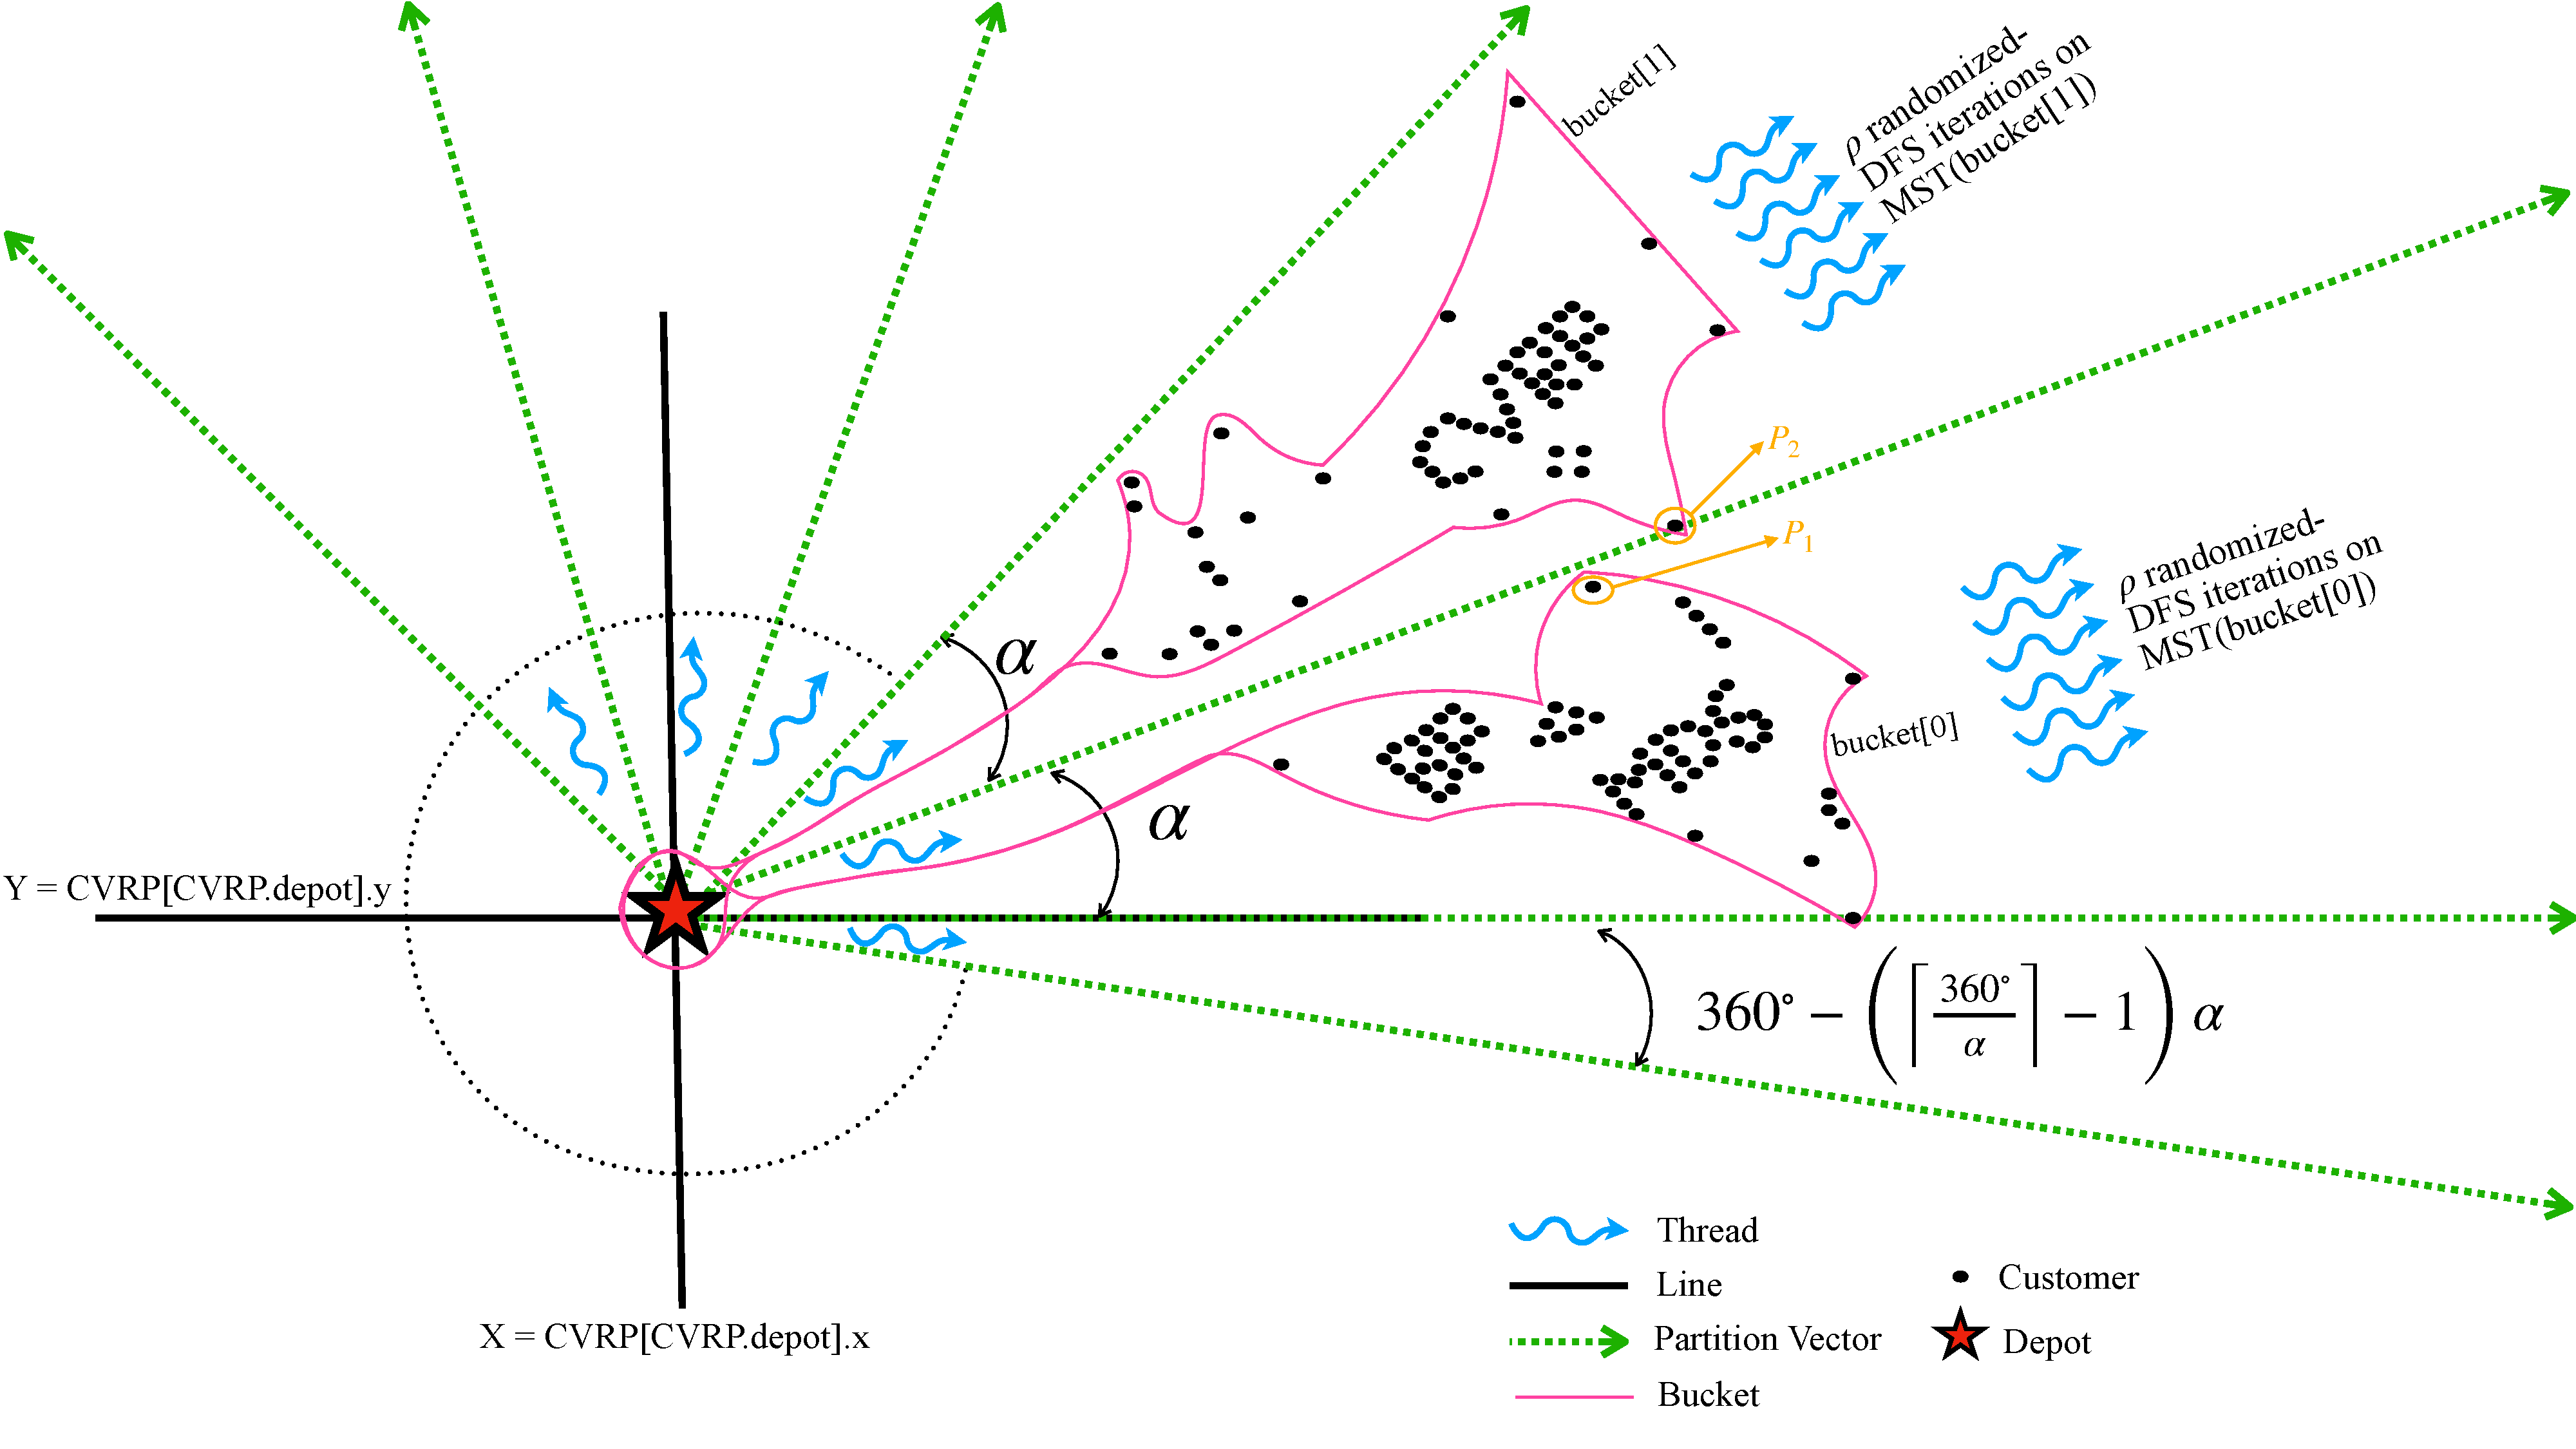
\includegraphics[width=\textwidth, height=0.45\textheight, keepaspectratio]{assets/2-d-partitions-refined.pdf}
    \caption{2-D partitioning in BP-MDS}
    \label{fig:2-d-partition}
\end{figure*}

\section{Background and Related Work}
\label{sec::background}

In CVRP, we are given a depot and $(N-1)$ customer nodes. Each node $id \in \{0, 1, \dots, \allowbreak N-1\}$ is associated with coordinates\\$(CVRP[id].x,\allowbreak\ CVRP[id].y)$ in the 2D Euclidean plane, where the depot is identified by $id = 0$. Each customer node $id$ has an associated demand $CVRP[id].demand$ satisfying $0 < CVRP[id].demand \leq Q$, where $Q$ denotes the capacity of each vehicle. The depot has zero demand. A fleet of identical vehicles, each with capacity $Q$, is stationed at the depot, and the fleet size is assumed to be sufficiently large to serve all customers. The cost between any pair of nodes is defined as the Euclidean distance between their corresponding coordinates. The objective is to determine a set of routes such that each route starts and ends at the depot, each customer is visited exactly once, and the total demand served in any route does not exceed the vehicle capacity $Q$, while minimizing the total travel cost. A CVRP instance can be modeled as a complete weighted graph $G = (V, E)$, where $V$ denotes the set of nodes, $E$ the set of edges, and edge weights represent pairwise distances between nodes.

State-of-the-art solutions for medium-scale CVRP instances are typically obtained using metaheuristics such as Genetic Algorithms, Tabu Search, and Hybrid Genetic Search (HGS)~\cite{vidal2012hybrid}, which are highly effective in reducing the optimality gap and often achieve near-optimal solutions. A significant body of research has also focused on designing heuristic and metaheuristic approaches that trade optimality for computational efficiency~\cite{Toth_VRP}, including classical methods such as the Clarke--Wright savings algorithm~\cite{Clarke_Wright} and sweep-based heuristics~\cite{Sweep_Heuristic}, which exploit geometric properties to construct feasible routes efficiently. More recent advances combine local search with powerful diversification strategies to further improve solution quality~\cite{vidal2022hybrid}. However, despite their effectiveness on benchmark datasets, these approaches remain computationally intensive and exhibit limited scalability when applied to instances with hundreds of thousands or millions of nodes, with execution time and memory requirements posing significant challenges.

With the rise of multi-core and high-performance computing systems, parallel approaches to CVRP have gained traction. These methods distribute either the search process or the problem structure across processing units. Crainic~\cite{crainic2006parallel} introduced an early and influential parallel metaheuristic that explores multiple solution trajectories concurrently. Despite their effectiveness, such approaches often incur synchronization overhead and exhibit limited scalability due to shared data structures. Tree-based heuristics, especially those based on Minimum Spanning Trees (MSTs), are widely used in routing due to their ability to capture the graph structure efficiently. MST-based methods are computationally light and often serve as a backbone for constructing feasible tours~\cite{CLRS}. Combining spanning trees with traversal strategies such as depth-first search~(DFS) enables the generation of approximate solutions with linear or near-linear time and low memory overhead, making them suitable for large-scale instances. ParMDS~\cite{Muniasamy_VRP} follows this paradigm by constructing an MST over the complete CVRP graph and exploring multiple randomized DFS traversals to generate diverse route sets. While effective, its scalability is limited to approximately $5\times 10^4$ customers in the input instance.

Our work builds upon these directions by combining spatial decomposition with tree-based route construction in a parallel setting. Unlike classical metaheuristics that focus on solution optimality, our primary objective is to achieve scalable performance on massive CVRP instances. Compared to ParMDS~\cite{Muniasamy_VRP}, our approach introduces a lightweight angular partitioning scheme coupled with randomized exploration over MST structures, enabling efficient utilization of modern multi-core architectures. The proposed Bucket-Partitioned-MDS (BP-MDS) framework is designed to balance solution quality, execution time, and memory usage, making it suitable for million-scale CVRP instances where traditional methods become impractical. Unlike single-threaded solvers such as \textsc{HGS-CVRP}, which primarily prioritize solution quality and are typically limited to instances with a few thousand customers, our proposed \textsc{BP-MDS} scales to million-customer problem instances and delivers orders-of-magnitude speedups.



\section{Our Approach}
\label{sec:approach}

\subsection{Motivation}
\label{sec:motivation}
Our primary motivation is to solve large-scale CVRP instances with competitive accuracy and reduced execution time. To achieve this, we leverage data structure optimizations, including a custom min-heap and on-demand memory allocation, along with parallelism provided by modern multi-core architectures. Fig.~\ref{fig:BKS_Brussels} illustrates the Best Known Solution (BKS) for the Brussels instances from CVRPLIB~\cite{CVRPLIB}. A notable structural pattern can be observed in the solution: routes exhibit a flower-like arrangement, where the depot acts as the center and individual routes resemble petals radiating outward. This geometric characteristic motivates a spatial decomposition strategy. Specifically, we partition the plane into triangular regions (or equivalently, two-dimensional cones) with the depot as the common vertex. Such a partitioning enables an effective distribution of computational workload. Thus, empirically, for most large instances, the load is approximately balanced across angular sectors, where each region can be assigned to a separate thread. This insight forms the basis of the proposed BP-MDS approach, illustrated in Fig.~\ref{fig:2-d-partition}. 

A key design choice in our approach is to avoid explicitly constructing the complete graph. For million-scale instances, materializing all edges is computationally prohibitive, particularly in terms of total available memory. Instead, we operate on the graph implicitly, computing edge weights on demand. This representation enables scalability without compromising the solution quality. To support efficient route construction, we explicitly maintain the Minimum Spanning Trees (MSTs), which can be stored compactly and form a core component of our CVRP framework.













\subsection{Core Algorithm}
\label{subsec::algorithm}

Algorithm~\ref{alg:bucket-cvrp} presents our Bucket-Partitioned MDS (BP-MDS), a divide-and-conquer parallel and memory-efficient algorithm. The method is governed by two key parameters: the angular partitioning parameter $\alpha$, which controls the number of spatial decompositions, and the exploration parameter $\rho$, which governs the diversity of route constructions. The algorithm takes these two parameters, $\alpha$ and $\rho$, as inputs and produces a feasible, high-quality approximate solution to the CVRP.

\textbf{Divide CVRP:} BP-MDS partitions the two-dimensional plane into angular regions (Line~\ref{alg:bucket-cvrp:line2}) centered at the depot. Customers are assigned to their respective regions based on their angular positions, and together with the depot, are grouped into buckets (Fig.~\ref{fig:2-d-partition}). This step is implemented via the \textsc{Get\_Buckets} procedure (Algorithm~\ref{alg:get-buckets}, detailed in Section~\ref{subsec:create_buckets}). Within each bucket, we conceptually model a complete graph over the assigned vertices without explicitly materializing all the edges.

\textbf{Conquer CVRP in Parallel:} BP-MDS processes each bucket independently in parallel (Lines~\ref{alg:bucket-cvrp:line3}--\ref{alg:bucket-cvrp:line22}), forming the core conquer phase of the algorithm. For every bucket, we construct a Minimum Spanning Tree (MST) over its vertices (Line~\ref{alg:bucket-cvrp:line4}) using \textsc{Construct\_MST} (Algorithm~\ref{alg:construct-mst}, detailed in Section~\ref{subsec:construct_mst}), which provides a sparse backbone for route generation. To explore diverse routing configurations, we perform $\rho$ independent iterations in parallel (Lines~\ref{alg:bucket-cvrp:line6}--\ref{alg:bucket-cvrp:line13}), each generating a candidate solution via a randomized depth-first traversal of the MST (Algorithm~\ref{alg:get-routes-from-random-dfs}, detailed in Section~\ref{subsec:routes_construction_via_random_DFS}). Within each partition, additional parallelism is exploited by spawning sub-threads to solve the corresponding subproblems using different route orderings induced by $\rho$. This results in a hierarchical (multi-level or nested) parallelization scheme. Among the generated candidates, the minimum-cost solution is selected for subsequent processing using a critical section (Line~\ref{alg:bucket-cvrp:line8}) to safely update the shared variables ($min\_cost\_routes$ and $min\_cost$).
Finally, the partial solutions obtained from all the partitions are refined (Line~\ref{alg:bucket-cvrp:line17}) through intra-route optimization using 2-opt~\cite{Croes_1958, Flood_1956} and the nearest-neighbor heuristics~\cite{Rosenkrantz_1977}, following the approach of Muniasamy et al.~\cite{Muniasamy_VRP} to improve the solution quality. These refined routes are then combined in a consolidation phase to construct a complete feasible solution in a critical section (Lines~\ref{alg:bucket-cvrp:line18}--\ref{alg:bucket-cvrp:line21}) %to avoid race conditions, 
as both the global route container and the total cost are shared across concurrently running worker threads. 



\begin{algorithm}
\caption{\textsc{Bucket\_Partitioned\_MDS}}
\label{alg:bucket-cvrp}
\SetEndCharOfAlgoLine{}
\SetAlgoLined

\KwIn{CVRP instance, parameters $\alpha$, $\rho$}
\KwOut{$routes$: feasible CVRP solution; $cost$: total cost}

$final\_routes \gets \emptyset$, $final\_cost \gets 0$\;  \label{alg:bucket-cvrp:line1}

\tcp{Divide CVRP}
$buckets \leftarrow \textsc{Get\_Buckets}(CVRP, \alpha)$  \label{alg:bucket-cvrp:line2}


\For{bucket in buckets \textbf{in parallel}} { \label{alg:bucket-cvrp:line3}

    $T \leftarrow \textsc{Construct\_MST}(CVRP, bucket)$\;                                              \label{alg:bucket-cvrp:line4}
    
    $min\_cost\_routes \leftarrow \emptyset$, $min\_cost \leftarrow \infty$\;                           \label{alg:bucket-cvrp:line5}
    
    \tcp{Exploit the MST by exploring multiple DFS orderings}
    \For{$\rho$ iterations \textbf{in parallel}}{  \label{alg:bucket-cvrp:line6}
        $(routes, cost) \leftarrow \textsc{Get\_Routes\_From\_Random\_DFS}(CVRP, T, bucket)$\; \label{alg:bucket-cvrp:line7}

        \Critical{                                                                                      \label{alg:bucket-cvrp:line8}
            \If{$cost < min\_cost$}{                                                                    \label{alg:bucket-cvrp:line9}
                $min\_cost\_routes \leftarrow routes$, $min\_cost \leftarrow cost$\;                                                           \label{alg:bucket-cvrp:line10}
            } \label{alg:bucket-cvrp:line11}
        } \label{alg:bucket-cvrp:line12}
    } \label{alg:bucket-cvrp:line13}

    \tcp{Refine and combine routes from all partitions}
    $(refined\_routes, refined\_cost) \leftarrow \textsc{Refine\_Routes}(CVRP, min\_cost\_routes)$\;    \label{alg:bucket-cvrp:line17}
    \Critical{                                                                                          \label{alg:bucket-cvrp:line18}
        $final\_routes \leftarrow final\_routes \cup refined\_routes$\;                                 \label{alg:bucket-cvrp:line19}
        $final\_cost \leftarrow final\_cost + refined\_cost$\;                                          \label{alg:bucket-cvrp:line20}
    }                                                                                                   \label{alg:bucket-cvrp:line21}
}                                                                                                       \label{alg:bucket-cvrp:line22}
\Return{$(final\_routes, final\_cost)$}                                                                 \label{alg:bucket-cvrp:line23}

\end{algorithm}






% \begin{figure*}[htbp]
%     \centering
%     \caption{Multi-level Multi-threading}
%     \label{fig:multi-level-threading}
%     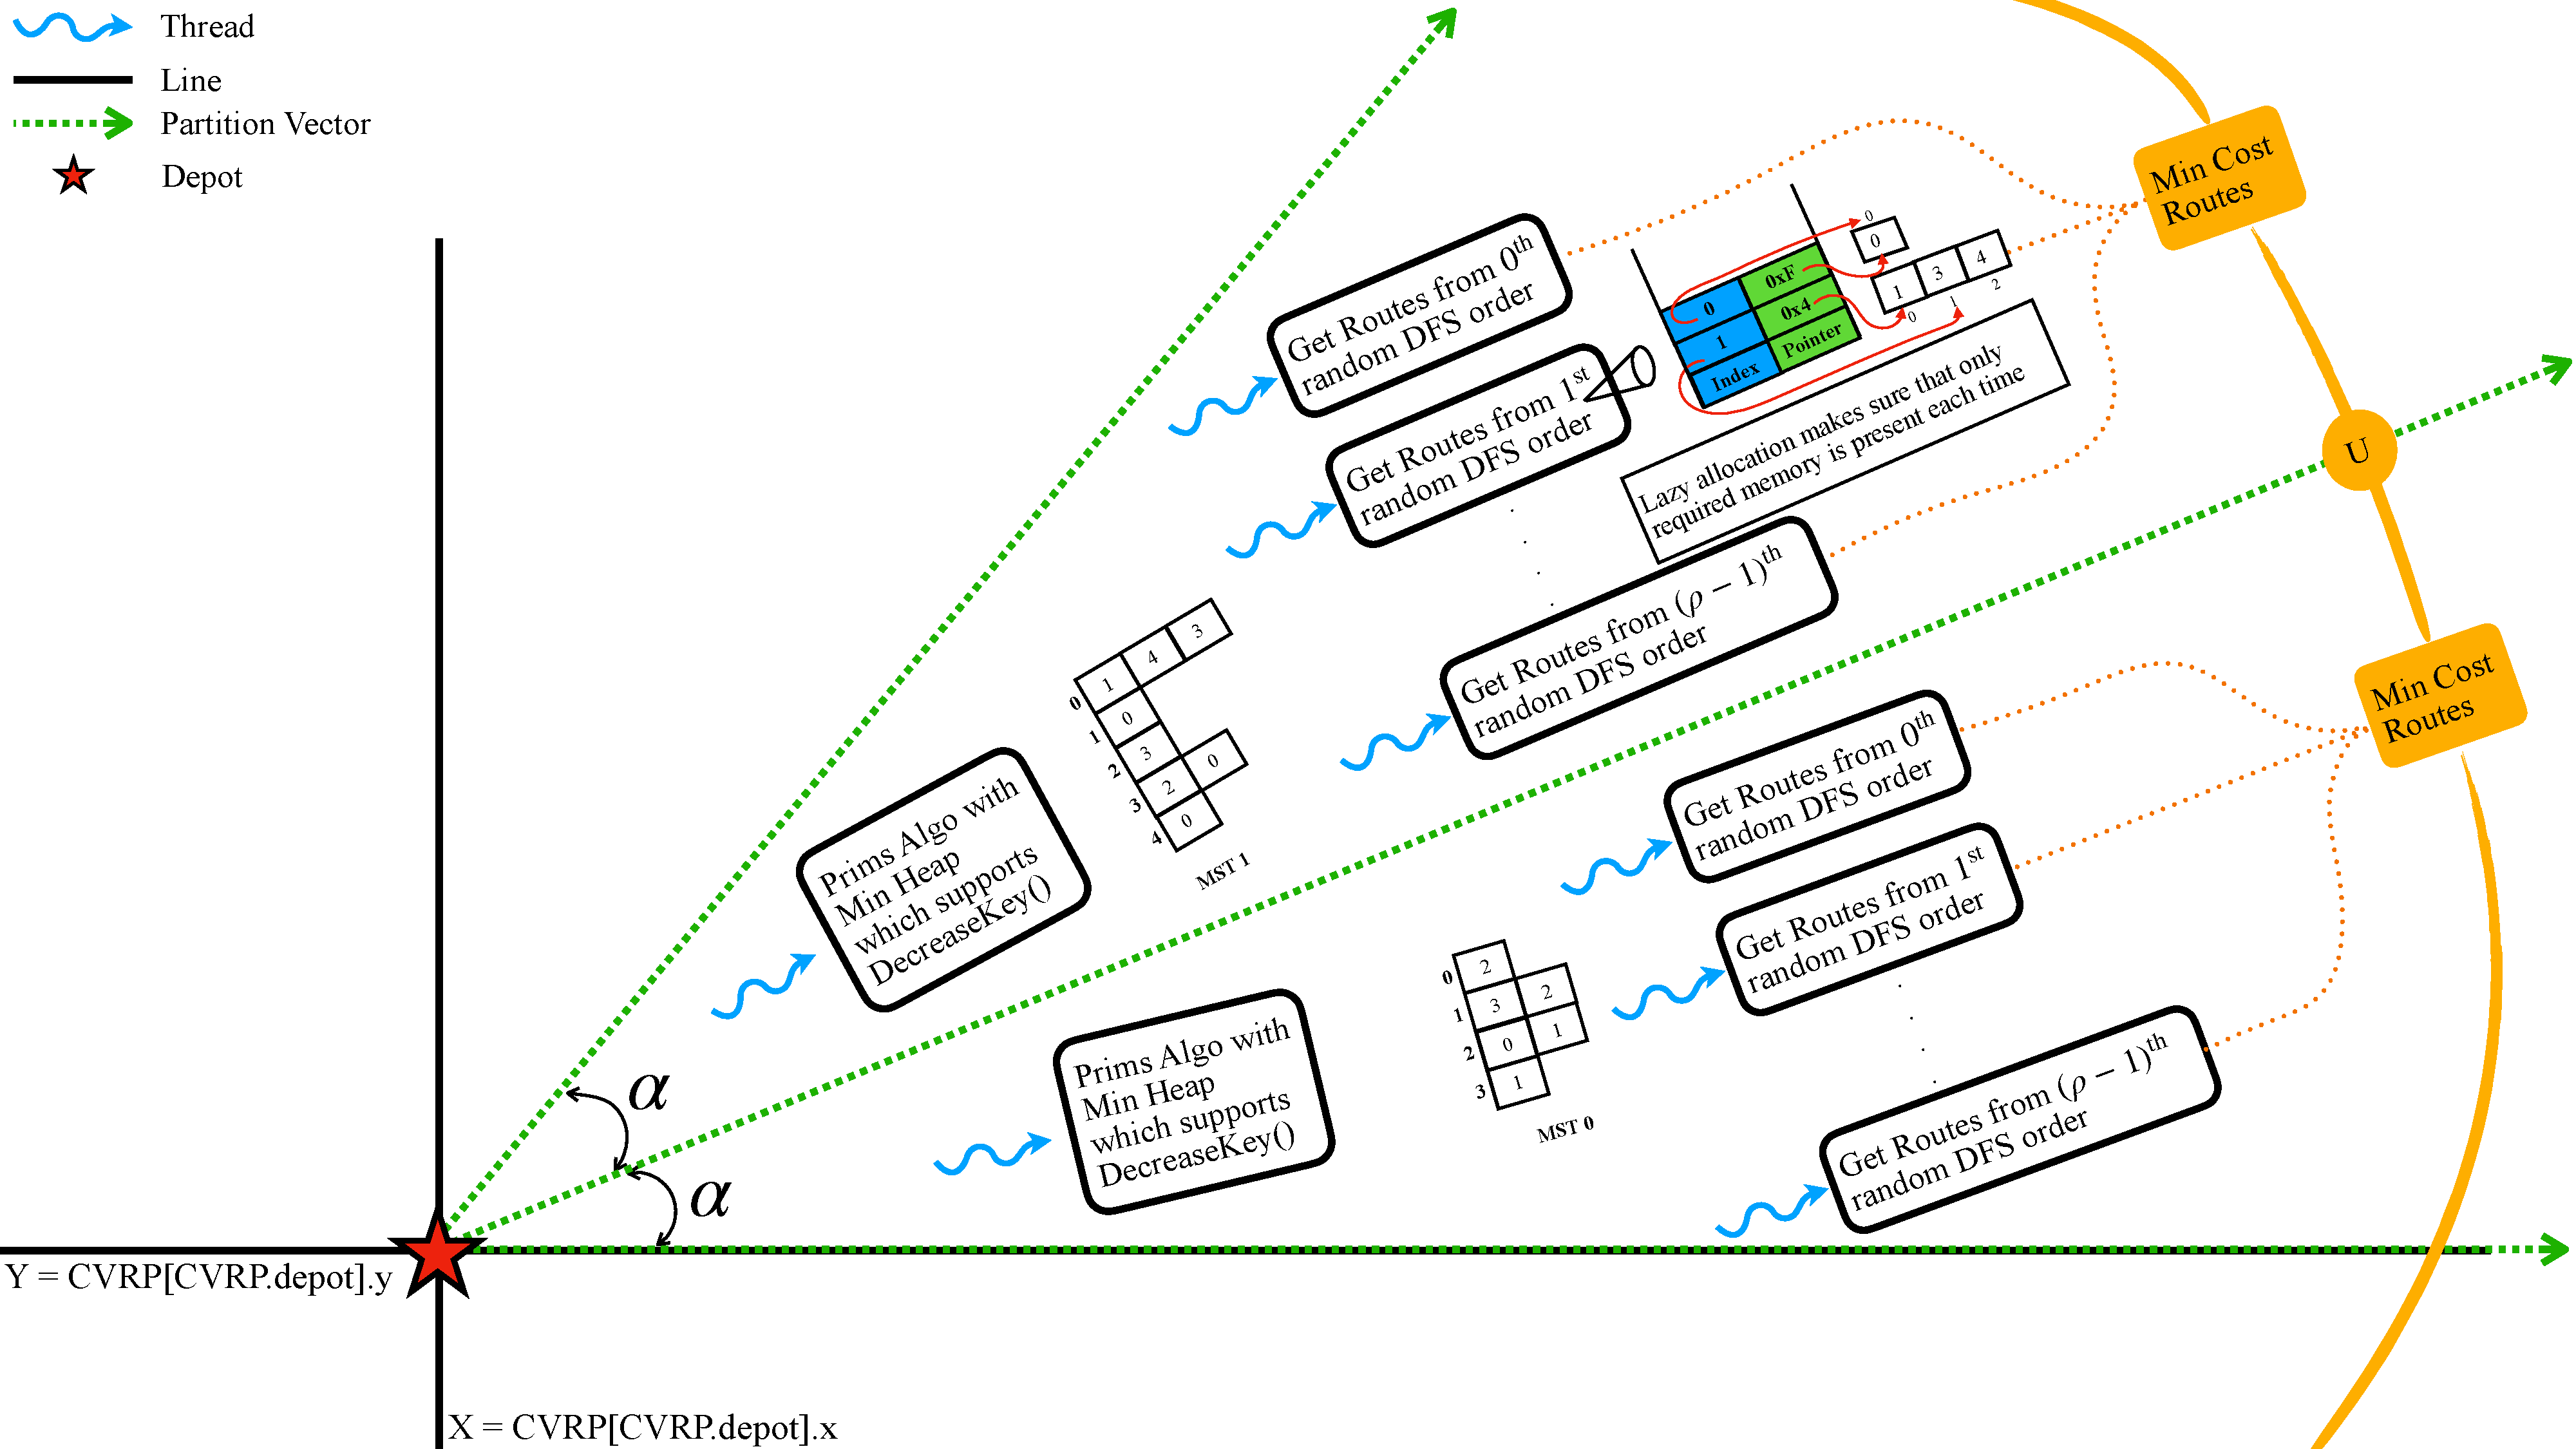
\includegraphics[width=\textwidth, height=0.4\textheight, keepaspectratio]{assets/multi-level-threading.pdf}
% \end{figure*}








\subsection{Create Buckets for CVRP instance}
\label{subsec:create_buckets}

Algorithm~\ref{alg:get-buckets} describes the partitioning of CVRP nodes into angular buckets based on their position relative to the depot. The \textsc{Get\_Buckets} procedure ensures that the depot is placed first in each bucket and each customer is assigned to exactly one bucket. A schematic illustration of this partitioning is provided in Fig.~\ref{fig:2-d-partition}. The number of buckets is computed as $k = \left\lceil \frac{360^\circ}{\alpha} \right\rceil$ (Line~\ref{alg:get-buckets:line1}), ensuring full coverage of the plane around the depot. To define the angular partition, we generate a sequence of unit vectors (Lines~\ref{alg:get-buckets:line2}--\ref{alg:get-buckets:line7}) corresponding to evenly spaced directions obtained by rotating a reference unit vector in increments of $\alpha$. These vectors induce a partition of the plane into $k$ contiguous angular sectors, as illustrated in Fig.~\ref{fig:2-d-partition}, where the partition vectors define the sector boundaries. For simplicity, we choose as the reference the horizontal line passing through the depot, i.e., the line $y=\texttt{CVRP[CVRP.depot].y}$, which is parallel to the positive $x$-axis. Accordingly, the reference unit vector is $\texttt{partition\_vectors}[0]=(1,0)$, and the remaining partition-defining unit vectors are generated by successive counterclockwise rotations of $\alpha$. Formally, for $i = 1, 2, \dots, k-1$, each vector satisfies $\text{partition\_vectors}[i] = \textsc{Rotate}_{\mathrm{CCW}}(\text{partition\_vectors}[0], i\alpha)$. Finally, $\text{partition\_vectors}[k] \allowbreak = \text{partition\_vectors}[0]$ completes the circular partition. Note that the last angular sector may have angular measure less than $\alpha$ when $\frac{360^\circ}{\alpha}$ is not an integer. The algorithm can be equivalently formulated using any fixed reference direction. The depot is inserted as the first element in every bucket to ensure that each subproblem constitutes a valid CVRP instance with a common starting point (Line~\ref{alg:get-buckets:line8}). Subsequently, each customer is assigned to exactly one bucket (Lines~\ref{alg:get-buckets:line9}--\ref{alg:get-buckets:line17}) based on the angular sector containing the unit vector from the depot, determined using the counterclockwise ordering of partition vectors. The use of half-open intervals (Line~\ref{alg:get-buckets:line12}) ensures that the partition is both disjoint and exhaustive, assigning every customer, including boundary points, unambiguously to a unique bucket. As illustrated in Fig.~\ref{fig:2-d-partition}, a point $P_1$ strictly within $[\text{partition\_vectors}[0],\, \allowbreak \text{partition\_vectors}[1])_{\text{CCW}}$ is assigned to $\text{bucket}[0]$, whereas a point $P_2$ lying exactly on \allowbreak $\text{partition\_vectors}[1]$ is assigned to $\text{bucket}[1]$. Once the appropriate bucket is identified, \texttt{break} (Line~\ref{alg:get-buckets:line14}) immediately terminates the search, avoiding unnecessary comparisons.



\begin{algorithm}[htbp]
\caption{\textsc{Get\_Buckets}}
\label{alg:get-buckets}
\SetAlgoLined
\SetEndCharOfAlgoLine{}

\KwIn{CVRP instance, angular partition parameter $\alpha \in (0,360^\circ]$}
\KwOut{Buckets}

\tcp{Compute the number of buckets}
$k \leftarrow \left\lceil \frac{360^\circ}{\alpha} \right\rceil$\;                                                  \label{alg:get-buckets:line1}

\tcp{Generate $k+1$ partition-defining unit vectors}
$partition\_vectors \leftarrow$ List of size $(k + 1)$\;                                                            \label{alg:get-buckets:line2}
$partition\_vectors[0] \leftarrow (1,0)$\;                                                                          \label{alg:get-buckets:line3}
\For{$i \leftarrow 1$ \KwTo $k - 1$}{                                                                               \label{alg:get-buckets:line4}
    $partition\_vectors[i] \leftarrow \textsc{Rotate}_{\mathrm{CCW}}(partition\_vectors[0],\, i \cdot \alpha)$\;    \label{alg:get-buckets:line5}
}                                                                                                                   \label{alg:get-buckets:line6}
$partition\_vectors[k] \leftarrow partition\_vectors[0]$\;                                                          \label{alg:get-buckets:line7}

\tcp{Insert depot first; Assign each customer to an angular bucket}
$buckets[i] \leftarrow [CVRP.depot],\ \forall\, i \in [0, k)$\;                                                     \label{alg:get-buckets:line8}
\For{$u \in \texttt{CVRP.customers}$}{                                                                              \label{alg:get-buckets:line9}
    $\mathbf{vec}_{du} \leftarrow$ unit vector from $CVRP.depot$ to $u$\;                                           \label{alg:get-buckets:line10}

    \For{$i \leftarrow 0$ \KwTo $k-1$}{                                                                             \label{alg:get-buckets:line11}  
        \If{$\mathbf{vec}_{du} \in [\,partition\_vectors[i],\, partition\_vectors[i+1])_{\text{CCW}}$}{             \label{alg:get-buckets:line12}
            $buckets[i].\text{push\_back}(u)$\;                                                                     \label{alg:get-buckets:line13}
            \textbf{break}\;                                                                                        \label{alg:get-buckets:line14}
        }                                                                                                           \label{alg:get-buckets:line15}
    }                                                                                                               \label{alg:get-buckets:line16}
}                                                                                                                   \label{alg:get-buckets:line17}

\Return{$buckets$}\;                                                                                                \label{alg:get-buckets:line18}

\end{algorithm}


\subsection{MST Construction}
%\subsection{Minimum Spanning Tree (MST) Construction}
\label{subsec:construct_mst}
For each bucket generated during the partitioning phase (Section~\ref{subsec:create_buckets}), we construct an MST over the corresponding subset of nodes. The MST is constructed using a variant of Prim’s algorithm, adapted to operate efficiently on the bucketed representation of the CVRP instance (Algorithm~\ref{alg:construct-mst}). Table~\ref{table:heap-operations} summarizes the min-heap operations used by Algorithms~\ref{alg:extract-relax} and~\ref{alg:construct-mst} for MST construction. The MST and the associated min-heap are constructed over the indices of vertices within a bucket, rather than their original CVRP node identifiers. This design enables the independent construction of an MST for each bucket, facilitating parallel execution in subsequent stages of the BP-MDS algorithm, where threads operate on these per-bucket MSTs without interference. Accordingly, variables such as $u\_index$, $v\_index$, and $depot\_index$ denote the positions of vertices $u$, $v$, and the $depot$ within the bucket. Algorithm~\ref{alg:extract-relax} extracts the minimum-weight edge from the min-heap and explores all neighbors of $v$ within the bucket. It then performs \textsc{DecreaseKey} operations to update the candidate edges, thereby maintaining the minimum-cost connections between vertices already in the MST and those not yet included. 

\begin{table}[htbp]
\centering
\caption{Min-Heap Operations used for MST Construction}
\label{table:heap-operations}
\begin{tabular}{l p{5cm}}
\toprule % Top thick line
\textbf{Operation} & \textbf{Description} \\
\midrule 

\textsc{Initialize}$(n)$ & Initializes a min-heap of capacity $n$ storing edges $(u, v, w)$, where $u, v$ are endpoints and $w$ is the weight. \\

\addlinespace 

\textsc{DecreaseKey}$(u, v, w)$ 
& Updates the key of vertex $v$ if the edge $(u, v)$ with weight $w$ provides a lower-cost connection. \\

\addlinespace

\textsc{Pop}$()$ 
& Removes and returns the element with the minimum weight. \\
\bottomrule % Bottom thick line
\end{tabular}
\end{table}

In Algorithm~\ref{alg:construct-mst}, the key of the depot in the min-heap is set to $0$ (Line~\ref{alg:construct-mst:line4}), while all other vertices are assigned a key of $\infty$. Consequently, the depot is extracted first (in Line~\ref{alg:construct-mst:line5}) and it serves as the starting point for MST construction. At each iteration (Lines~\ref{alg:construct-mst:line6}--\ref{alg:construct-mst:line10}), the algorithm extracts the minimum-weight edge $(u\_index, v\_index)$ from the heap, where $v\_index$ corresponds to a vertex not yet included in the MST. The edges incident to $v\_index$ are relaxed, updating the candidate connections. The selected edge is subsequently added to the MST by updating the adjacency list (Lines~\ref{alg:construct-mst:line8}--\ref{alg:construct-mst:line9}). This process continues until all vertices in the bucket are incorporated into the MST.

\begin{algorithm}[t]
\caption{\textsc{Extract\_Min\_And\_Relax\_Edges}}
\label{alg:extract-relax}
\SetAlgoLined
\SetEndCharOfAlgoLine{}

\KwIn{MinHeap $H$, CVRP instance $CVRP$, vertex list $bucket$}
\KwOut{Indices $(u\_index, v\_index)$ corresponding to extracted edge}

$(u\_index,\ v\_index,\ weight) \gets H.\textsc{Pop}()$\;     \label{alg:extract-relax:line1}
$v \gets bucket[v\_index]$\;                                  \label{alg:extract-relax:line2}

\tcp{Relax edges from $v\_index$ to all remaining vertices in bucket}
\For{$w\_index \gets 0$ \KwTo $|bucket| - 1$}{                 \label{alg:extract-relax:line3}
    $w \gets bucket[w\_index]$\;                              \label{alg:extract-relax:line4}
    $H.\textsc{DecreaseKey}(v\_index,w\_index,CVRP.distance(v,\ w))$\;\label{alg:extract-relax:line5}
}

\Return{$(u\_index,\ v\_index)$}\;                             \label{alg:extract-relax:line6}

\end{algorithm}

\begin{algorithm}[t]
\caption{\textsc{Construct\_MST}}
\label{alg:construct-mst}
\SetAlgoLined
\SetEndCharOfAlgoLine{}

\KwIn{CVRP instance $CVRP$, vertex bucket $bucket$}
\KwOut{Adjacency list $T$ representing an MST over $bucket$}

$depot\_index \gets 0$\;                                                                        \label{alg:construct-mst:line1}
$T \gets$ adjacency list initialized with $|bucket|$ empty lists\;                              \label{alg:construct-mst:line2}
MinHeap $H.\textsc{Initialize}(|bucket|)$\;                                                     \label{alg:construct-mst:line3}

\tcp{Initialize Prim's algorithm from depot}
$H.\textsc{DecreaseKey}(NULL,\ depot\_index,\ 0)$\;                                             \label{alg:construct-mst:line4}
$\textsc{Extract\_Min\_And\_Relax\_Edges}(H,\ CVRP,\ bucket)$\;     \label{alg:construct-mst:line5}

\tcp{Iteratively grow the MST}
\While{$H$ not empty}{                                                                          \label{alg:construct-mst:line6}

    $(u\_index,\ v\_index) \gets \textsc{Extract\_Min\_And\_Relax\_Edges}(H,\ CVRP,\ bucket)$\; \label{alg:construct-mst:line7}

    \tcp{Add edge to MST}
    $T[u\_index].push\_back(v\_index)$\;                                                         \label{alg:construct-mst:line8}
    $T[v\_index].push\_back(u\_index)$\;                                                         \label{alg:construct-mst:line9}
}                                                                                                \label{alg:construct-mst:line10}

\Return{$T$}\;                                                                                   \label{alg:construct-mst:line11}

\end{algorithm}

\subsection{Route Construction: Randomized Lazy DFS}
\label{subsec:routes_construction_via_random_DFS}
Algorithm~\ref{alg:get-routes-from-random-dfs} generates feasible CVRP routes from the MST via randomized DFS, using the traversal order while enforcing capacity-based splits. A stack-based DFS is used, where each element $(i, L)$ tracks the current index in a shuffled neighbor list (Line~\ref{alg:get-routes-from-random-dfs:line4}). Standard stack operations \textsc{PUSH}, \textsc{TOP}, and \textsc{POP} are employed. The traversal is initialized from the depot node, whose neighbors in the MST are randomly permuted to induce variability in the traversal order (Lines~\ref{alg:get-routes-from-random-dfs:line6}--\ref{alg:get-routes-from-random-dfs:line9}). At Line~\ref{alg:get-routes-from-random-dfs:line6}, we create a local copy of the adjacency list rather than directly shuffling the tree $T$, since $T$ is a shared data structure accessed by multiple threads. Each thread independently copies the neighbor list, performs a random permutation (Line~\ref{alg:get-routes-from-random-dfs:line7}), and then pushes the pair $(|L|-1, L)$ onto the stack (Line~\ref{alg:get-routes-from-random-dfs:line8}). This enables traversal from the end, with a simple termination condition: when the index becomes negative, all neighbors have been visited.

The algorithm proceeds by iteratively exploring the MST using the stack (Line~\ref{alg:get-routes-from-random-dfs:line10}). At each step, the top stack frame is examined, and unvisited neighbors are considered in reverse order of the shuffled list. Upon encountering an unvisited vertex $v$, the algorithm first checks whether adding $v$ to the current route would violate the vehicle capacity constraint (Line~\ref{alg:get-routes-from-random-dfs:line18}). If the constraint is violated, the current route is finalized by returning to the depot, and a new route is initiated (Lines~\ref{alg:get-routes-from-random-dfs:line19}--\ref{alg:get-routes-from-random-dfs:line22}). If the capacity constraint is satisfied, the vertex $v$ is appended to the current route, and the traversal cost is updated accordingly (Lines~\ref{alg:get-routes-from-random-dfs:line24}--\ref{alg:get-routes-from-random-dfs:line27}). The vertex is then marked as visited, and its neighbors are retrieved, copied, shuffled, and pushed onto the stack to continue the DFS exploration (Lines~\ref{alg:get-routes-from-random-dfs:line28}--\ref{alg:get-routes-from-random-dfs:line31}). Once all neighbors have been visited, the vertex is popped from the stack (Line~\ref{alg:get-routes-from-random-dfs:line35}); otherwise, the next neighbor index is updated to resume exploration after backtracking to the vertex (Line~\ref{alg:get-routes-from-random-dfs:line36}). Any remaining partial route is finalized by returning to the depot (Lines~\ref{alg:get-routes-from-random-dfs:line39}--\ref{alg:get-routes-from-random-dfs:line42}). The key features of the algorithm are: (i) on-demand (lazy) memory allocation, (ii) an iterative design, and (iii) on-the-fly distance computation for route construction.



\begin{algorithm}[htbp]
\caption{\textsc{Get\_Routes\_From\_Random\_DFS}}
\label{alg:get-routes-from-random-dfs}
\SetAlgoLined
\SetEndCharOfAlgoLine{}

\KwIn{CVRP instance: $CVRP$, Bucket of nodes: $bucket$, MST adjacency list over $bucket$: $T$}
\KwOut{List of routes: $routes$, Cost of routes: $cost$}

$num\_nodes \gets |bucket|$, $depot\_index \gets 0$\;                                                                       \label{alg:get-routes-from-random-dfs:line1}

$visited[0, \dots ,num\_nodes - 1] \gets false$\;                                                                           \label{alg:get-routes-from-random-dfs:line2}
$routes \gets [\ ]$,  $cost \gets 0$, $curr\_route \gets [\ ]$\;                                                            \label{alg:get-routes-from-random-dfs:line3}

$dfs\_stack \gets$ empty stack of $(i, L)$, where $i$ indexes into a neighbor list referenced by $L$\;                      \label{alg:get-routes-from-random-dfs:line4}
$residue\_capacity \gets CVRP.capacity$, $prev\_node \gets CVRP.depot$\;                                                    \label{alg:get-routes-from-random-dfs:line5}

\tcp{Start DFS from $depot\_index$}
$neigh \gets$ Copy($T[depot\_index]$)\;                                                                                     \label{alg:get-routes-from-random-dfs:line6}
\textsc{Shuffle}$(neigh)$\;                                                                                                 \label{alg:get-routes-from-random-dfs:line7}
$dfs\_stack.\textsc{Push}((|neigh|-1,\ neigh))$\;                                                                           \label{alg:get-routes-from-random-dfs:line8}
$visited[depot\_index] \gets true$\;                                                                                        \label{alg:get-routes-from-random-dfs:line9}

\While{$dfs\_stack$ is not empty}{                                                                                          \label{alg:get-routes-from-random-dfs:line10}
    $(index, neigh) \gets dfs\_stack.\textsc{Top}()$\;                                                                      \label{alg:get-routes-from-random-dfs:line11}
    $push\_candidate \gets NULL$\;                                                                                          \label{alg:get-routes-from-random-dfs:line12}

    \While{$index \geq 0$}{                                                                                                 \label{alg:get-routes-from-random-dfs:line13}
        $v\_index \gets neigh[index]$\;                                                                                     \label{alg:get-routes-from-random-dfs:line14}
        $v \gets bucket[v\_index]$\;                                                                                        \label{alg:get-routes-from-random-dfs:line15}
        $index \gets index - 1$\;                                                                                           \label{alg:get-routes-from-random-dfs:line16}

        \If{not $visited[v\_index]$}{                                                                                       \label{alg:get-routes-from-random-dfs:line17}

            \tcp{Start new route if the capacity is exceeded}                             
            \If{$residue\_capacity < CVRP[v].demand$}{                                                                      \label{alg:get-routes-from-random-dfs:line18}
                $routes.push\_back(curr\_route)$\;                                                                          \label{alg:get-routes-from-random-dfs:line19}
                $cost \gets cost + CVRP.distance(prev\_node, CVRP.depot)$\;                                                 \label{alg:get-routes-from-random-dfs:line20}
                $curr\_route \gets [\ ]$\;                                                                                  \label{alg:get-routes-from-random-dfs:line21}
                $residue\_capacity \gets CVRP.capacity$, $prev\_node \gets CVRP.depot$\;                                    \label{alg:get-routes-from-random-dfs:line22} 
            }                                                                                                               \label{alg:get-routes-from-random-dfs:line23}

            \tcp{Add $v$ to current route}
            $curr\_route.push\_back(v)$\;                                                                                   \label{alg:get-routes-from-random-dfs:line24}
            $cost \gets cost + CVRP.distance(prev\_node, v)$\;                                                              \label{alg:get-routes-from-random-dfs:line25}
            $residue\_capacity \gets residue\_capacity - CVRP[v].demand$\;                                                  \label{alg:get-routes-from-random-dfs:line26}
            $prev\_node \gets v$\;                                                                                          \label{alg:get-routes-from-random-dfs:line27}

            \tcp{DFS from $v\_index$}
            $visited[v\_index] \gets true$\;                                                                                \label{alg:get-routes-from-random-dfs:line28}
            $neigh' \gets$ Copy($T[v\_index]$)\;                                                                            \label{alg:get-routes-from-random-dfs:line29}
            \textsc{Shuffle}$(neigh')$\;                                                                                    \label{alg:get-routes-from-random-dfs:line30}
            $push\_candidate \gets (|neigh'|-1,\ neigh')$\;                                                                 \label{alg:get-routes-from-random-dfs:line31}

            \textbf{break}\;                                                                                                \label{alg:get-routes-from-random-dfs:line32}
        }                                                                                                                   \label{alg:get-routes-from-random-dfs:line33}
    }                                                                                                                       \label{alg:get-routes-from-random-dfs:line34}

    \lIf{$index < 0$}{$dfs\_stack.\textsc{Pop}()$ }                                                                         \label{alg:get-routes-from-random-dfs:line35}
    \lElse{$dfs\_stack.\textsc{Top}().first \gets index$ }                                                                  \label{alg:get-routes-from-random-dfs:line36}

    \lIf{$push\_candidate \neq NULL$}{$dfs\_stack.\textsc{Push}(push\_candidate)$ }                                         \label{alg:get-routes-from-random-dfs:line37}
}                                                                                                                           \label{alg:get-routes-from-random-dfs:line38}

\tcp{Add last route}
\If{$curr\_route \neq [\ ]$}{                                                                                               \label{alg:get-routes-from-random-dfs:line39}
    $routes.push\_back(curr\_route)$\;                                                                                      \label{alg:get-routes-from-random-dfs:line40}
    $cost \gets cost + CVRP.distance(prev\_node, CVRP.depot)$\;                                                             \label{alg:get-routes-from-random-dfs:line41}
}                                                                                                                           \label{alg:get-routes-from-random-dfs:line42}

\Return{$(routes,\ cost)$}\;                                                                                                \label{alg:get-routes-from-random-dfs:line43}

\end{algorithm}



% \subsection{Implementation}
% \label{subsec::implementation}
% \input{sections/Implementation}


\subsection{Theoretical Analysis}
\label{subsec::theoretical-analysis}



% \begin{table*}[t]
% \centering
% \small
% \caption{Per-instance results of BP-MDS ($\rho = 10^4$).}
% \label{tab:bpmds_per_instance_results}
% \begin{tabular}{|c|c|c|c|c|c|c|c|c|}
% \hline
% Class & N & Input & BKS & $\alpha$ ($^\circ$) & Time(s) & Memory(MB) & Cost & Gap(\%)\\
% \hline
% \noalign{\vskip 2pt} 
% \multirow{3}{*}{S} 
%  & 151 & CMT4 & 1028.42 & 127.0 & 0.0395 & 9.113 & 1143.98 & 11.23 \\
%  & 241 & Golden\_17 & 707.76 & 36.0 & 0.07 & 10.52 & 762.71 & 7.76 \\
%  & 301 & Golden\_18 & 995.13 & 24.0 & 0.12 & 14.88 & 1044.63 & 4.97 \\
% \hline

% \noalign{\vskip 2pt}
% \multirow{5}{*}{M} 
%  & 3001 & Leuven1 & 192848 & 30.0 & 0.302 & 10.26 & 207573.35 & 7.64 \\
%  & 4001 & Leuven2 & 111391 & 66.0 & 3.0 & 10.26 & 127447.35 & 14.41 \\
%  & 6001 & Antwerp1 & 477277 & 18.0 & 3.28 & 51.85 & 510570.898 & 6.97 \\
%  & 7001 & Antwerp2 & 291350 & 39.0 & 1.597 & 9.76 & 327747.64 & 12.49 \\
%  & 10001 & Ghent1 & 469531 & 23.0 & 0.78 & 10.41 & 503565.34 & 7.25 \\
% \hline

% \noalign{\vskip 2pt}
% \multirow{7}{*}{L} 
%  & 11001 & Ghent2 & 257749 & 35.5 & 2.04 & 10.26 & 292125.24 & 13.34 \\
%  & 15001 & Brussels1 & 501719 & 11.5 & 1.01 & 228.58 & 544650.63 & 8.56 \\
%  & 16001 & Brussels2 & 345481 & 31.0 & 2.25 & 9.75 & 390855.84 & 11.61 \\
%  & 20001 & Flanders1 & 7240124 & 18.0 & 1.34 & 11.47 & 7668875.48 & 5.92 \\
%  & 30001 & Flanders2 & 4373320 & 19.5 & 4.65 & 12.38 & 4864684.64 & 11.24 \\
%  & 25001 & XML25000\_1173\_01 & -- & 2.0 & 2.31 & 346.74 & 46902788.87 & -- \\
%  & 50001 & XML50000\_2173\_01 & -- & 2.5 & 5.04 & 343.13 & 58108045.17 & -- \\
% \hline

% \noalign{\vskip 2pt}
% \multirow{2}{*}{XL} 
%  & 75001 & XML75000\_1173\_01 & -- & 1.0 & 5.87 & 331.14 & 141858875.48 & \textunderscore{} \\
%  & 100001 & XML100000\_2173\_01 & -- & 1.0 & 9.73 & 333.01 & 116740181.51 & \textunderscore{} \\
% \hline

% \noalign{\vskip 2pt}
% \multirow{2}{*}{XXL}
%  & 500001 & XML500000\_1173\_01 & -- & 0.3 & 40.98 & 315.07 & 946129677.99 & \textunderscore{} \\
%  & 1000001 & XML1000000\_2123\_01 & -- & 0.3 & 88.67 & 288.31 & 993950684.86 & \textunderscore{} \\
% \hline

% \noalign{\vskip 2pt}
% \multirow{4}{*}{XXXL}
%  & 2000001 & XML2000000\_2121\_01 & -- & 0.2 & 204.04 & 298.89 & 5920305652.53 & \textunderscore{} \\
%  & 2000001 & XML2000000\_2123\_01 & -- & 0.2 & 172.03 & 274.20 & 1985907542.13 & \textunderscore{} \\
%  & 5000001 & XML5000000\_1173\_01 & -- & 0.1 & 458.98 & 219.36 & 2537203464.83 & \textunderscore{} \\
%  & 5000001 & XML5000000\_2176\_01 & -- & 0.1 & 492.73 & 238.55 & 1573789826.68 & \textunderscore{} \\
% \hline
% \end{tabular}
% \end{table*}

\begin{table*}[t]
\caption{Per-instance results of BP-MDS ($\rho = 10^4$).}
\centering
\small
\begin{tabular}{clrrrrrrr}
\toprule
Class & Input & N & BKS & $\alpha$ ($^\circ$) & Time (s) & Memory (MB) & Cost & Gap (\%)\\
\midrule
\multirow{2}{*}{S}
 & Golden\_17 & 241 & 707.76 & 36.0 & 0.07 & 10.52 & 762.71 & 7.76 \\
 & Golden\_18 & 301 & 995.13 & 24.0 & 0.12 & 14.88 & 1044.63 & 4.97 \\
\midrule
\multirow{5}{*}{M}
 & Leuven1 & 3001 & 192848 & 30.0 & 0.49 & 10.26 & 207573.35 & 7.64 \\
 & Leuven2 & 4001 & 111391 & 66.0 & 0.78 & 10.26 & 127544.83 & 14.50 \\
 & Antwerp1 & 6001 & 477277 & 18.0 & 0.53 & 51.85 & 512064.59 & 7.29 \\
 & Antwerp2 & 7001 & 291350 & 39.0 & 0.64 & 9.76 & 328377.84 & 12.71 \\
 & Ghent1 & 10001 & 469531 & 23.0 & 0.78 & 10.41 & 503730.90 & 7.28 \\
\midrule
\multirow{7}{*}{L}
 & Brussels1 & 15001 & 501719 & 11.5 & 1.01 & 175.10 & 544650.63 & 8.56 \\
 & Brussels2 & 16001 & 345468 & 31.0 & 2.25 & 9.75 & 390855.84 & 13.14 \\
 & Flanders1 & 20001 & 7240118 & 18.0 & 1.34 & 11.47 & 7668875.48 & 5.92 \\
 & Flanders2 & 30001 & 4373244 & 19.5 & 4.65 & 12.38 & 4864684.64 & 11.24 \\
 & XML25000\_1173\_01 & 25001 & -- & 2.0 & 2.31 & 346.74 & 46902788.87 & -- \\
 & XML50000\_2173\_01 & 50001 & -- & 2.5 & 5.04 & 343.13 & 58108045.17 & -- \\
 & Molise & 50000 & 111184982 & 23.0 & 3.35 & 19.83 & 113367183.12 & 1.96 \\
\midrule
\multirow{3}{*}{XL}
 & XML75000\_1173\_01 & 75001 & -- & 1.0 & 5.87 & 331.14 & 141858875.48 & -- \\
 & XML100000\_2173\_01 & 100001 & -- & 1.0 & 9.73 & 333.01 & 116740181.51 & -- \\
 & Trentino-Alto-Adige & 100000 & 102063181 & 34.0 & 14.52 & 34.24 & 104219633.59 & 2.11 \\
\midrule
\multirow{4}{*}{XXL}
 & Sardegna & 470000 & 827934149 & 15.0 & 132.33 & 78.73 & 828568977.54 & 0.08 \\
 & XML500000\_1173\_01 & 500001 & -- & 0.3 & 40.98 & 315.07 & 946129677.99 & -- \\
 & XML1000000\_2123\_01 & 1000001 & -- & 0.3 & 88.67 & 288.31 & 993950684.86 & -- \\
 & Lazio & 1000000 & 3145381332 & 5.0 & 101.99 & 143.92 & 3189655809.43 & 1.41\\
\midrule
\multirow{3}{*}{XXXL}
 & XML2000000\_2123\_01 & 2000001 & -- & 0.2 & 172.03 & 274.20 & 1985907542.13 & -- \\
 & XML5000000\_1176\_01 & 5000001 & -- & 0.1 & 465.79 & 218.85 & 2537175956.58 & -- \\
 & XML5000000\_2176\_01 & 5000001 & -- & 0.2 & 484.77 & 234.07 & 1573769553.19 & -- \\
\bottomrule
\end{tabular}

\label{tab:bpmds_per_instance_results}
\end{table*}


Let $k = \left\lceil \frac{360^\circ}{\alpha} \right\rceil$ denote the number of angular buckets. Let $\{s_0, s_1, \dots, \allowbreak s_{k-1}\}$ denote the sizes of the buckets, with $\sum_{j=0}^{k-1} s_j = N - 1 + k$, where the $N-1$ customers appear exactly once, while the depot is replicated across all $k$ buckets.

\textbf{Creation of Buckets:} The \textsc{Get\_Buckets} procedure assigns each of the $N-1$ customers to one of the $k$ buckets in $O((N-1)k)$ time, while bucket initialization and depot insertion require $O(k)$ time, yielding an overall time complexity of $O(Nk)$ and space complexity of $O(N + k)$.

\textbf{Per-Bucket Processing:} For a bucket of size $s_j$, MST construction (Prim’s with binary heap on an implicit complete graph) takes $O(s_j^2 \log s_j)$ time and $O(s_j)$ space. Each DFS-based route generation requires $O(s_j)$ time and space. Route refinement (e.g., 2-opt) costs $O(s_j^2)$ time and $O(s_j)$ space. 

$O\!\left(Nk + \sum_{j=0}^{k-1} \left( s_j^2 \log s_j + \rho\, s_j + s_j^2 \right)\right)$ is the overall time complexity in the sequential setting, while the space complexity is $O(N + k)$. Using the fact that $\sum_{j=0}^{k-1} s_j^2 \log s_j \le \left(\sum_{j=0}^{k-1} s_j\right)^2 \log\!\left(\sum_{j=0}^{k-1} s_j\right) = (N-1+k)^2 \log(N-1+k)$ (maximized when all the vertices lie in a single bucket), and noting that $k \ll N$, we obtain $\sum_{j=0}^{k-1} s_j^2 \log s_j = O(N^2 \log N)$. Hence, the overall sequential time complexity is upper bounded by $O(N^2 \log N)$, although this bound is conservative. In the parallel setting (assuming full parallelism), the overall time complexity is $O\!\left(Nk + \max_{0 \le j \le k-1} \left( s_j^2 \log s_j + s_j + s_j^2 \right)\right)$, where the execution time is dominated by the largest bucket.  For unbalanced buckets, the largest bucket becomes the bottleneck due to its $O(s_j^2 \log s_j)$ MST construction cost. Since the average bucket size is $\bar{s} = \frac{\sum_{j=0}^{k-1} s_j}{k} = \frac{N-1+k}{k} \approx \frac{N}{k}$, increasing $k$ reduces the average bucket size, thereby lowering the dominant per-bucket computation cost and improving parallel scalability. For approximately balanced buckets, i.e., $s_j \approx \frac{N}{k}$ for all $j$, $O\!\left(Nk + \frac{N^2}{k} \log \frac{N}{k} + \rho N  + \frac{N^2}{k} \right)$ is the sequential time complexity, while the parallel time complexity reduces to $O\!\left(Nk + \frac{N^2}{k^2} \log \frac{N}{k} + \frac{N}{k} + \frac{N^2}{k^2}\right)$. This demonstrates a near-$k$-fold reduction in the dominant quadratic term under full parallelism and eliminates the $\rho$ component. The running time decreases with increasing $k$, while the resulting increase in buckets enables greater parallelism, yielding strong scalability with increasing core counts.


% The running time decreases with increasing $k$, while the proportional increase in parallelism enables strong scalability with increasing core counts.

% The running time decreases with increasing $k$, while the degree of parallelism grows proportionally, as more buckets enable greater concurrency across threads. Consequently, the approach exhibits strong scalability with an increasing number of cores.


\section{Experimental Evaluation}
\label{sec::experimental-evaluation}

\subsection{BP-MDS Execution and Evaluation}

\begin{figure*}[t]
    \centering
    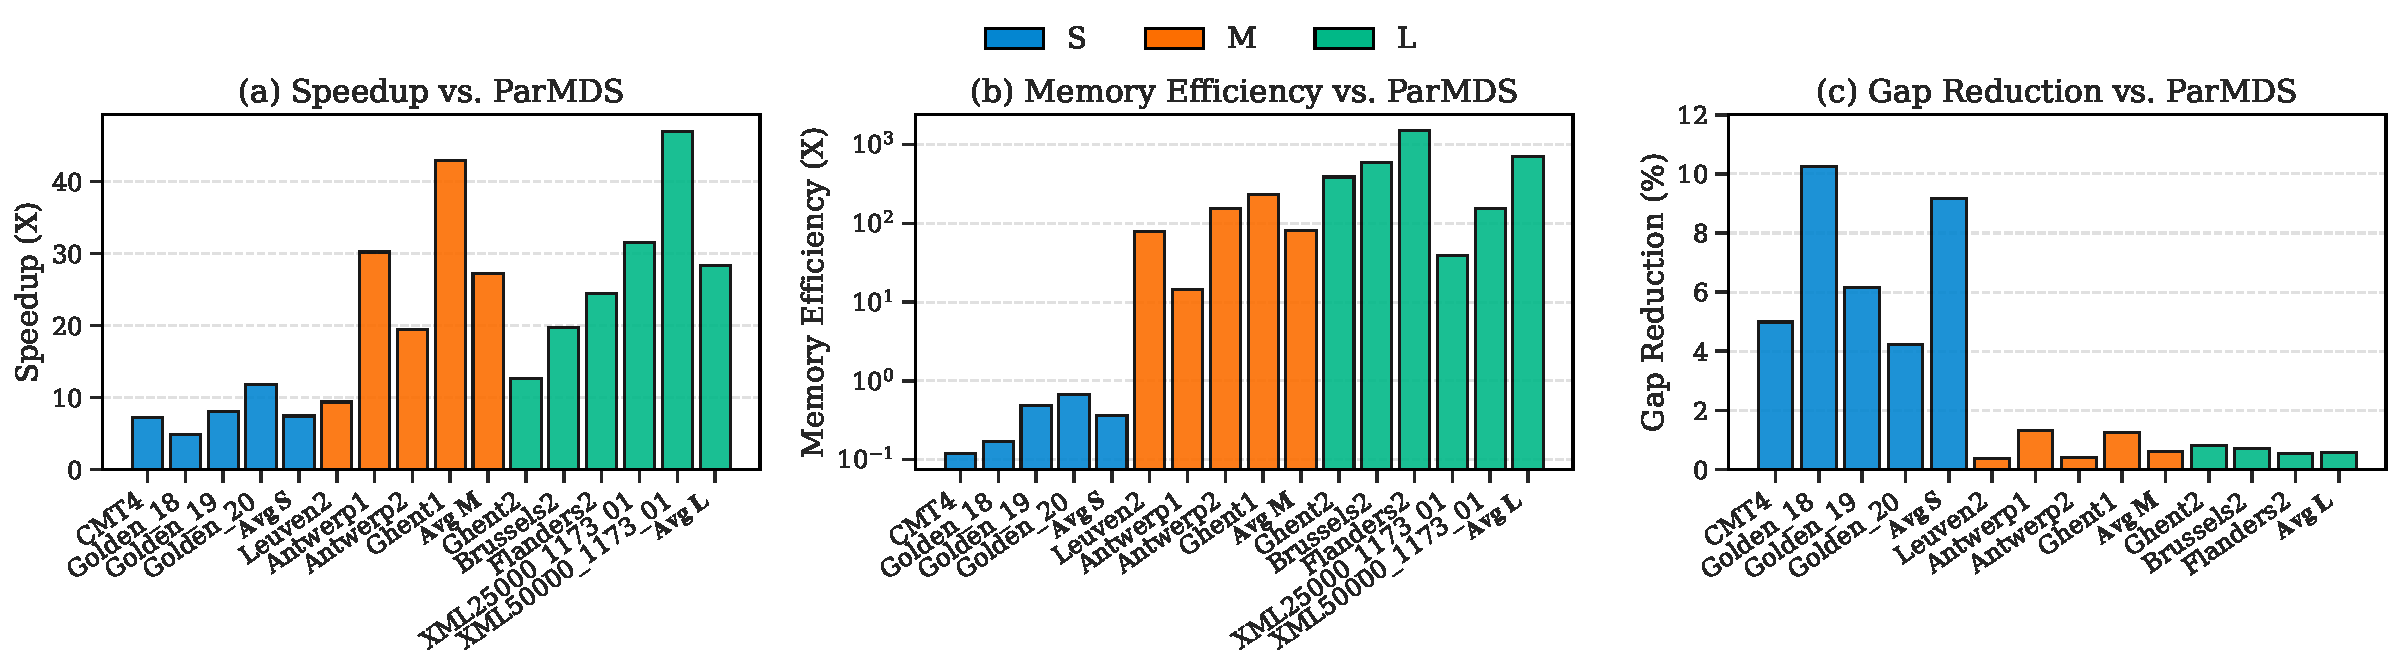
\includegraphics[width=\linewidth]{sections/results/parMDS.pdf}
    \caption{BP-MDS vs.\ ParMDS performance}
    \label{fig:parMDS_comparison_grid1}
\end{figure*}

\begin{figure*}[ht]
    \centering
    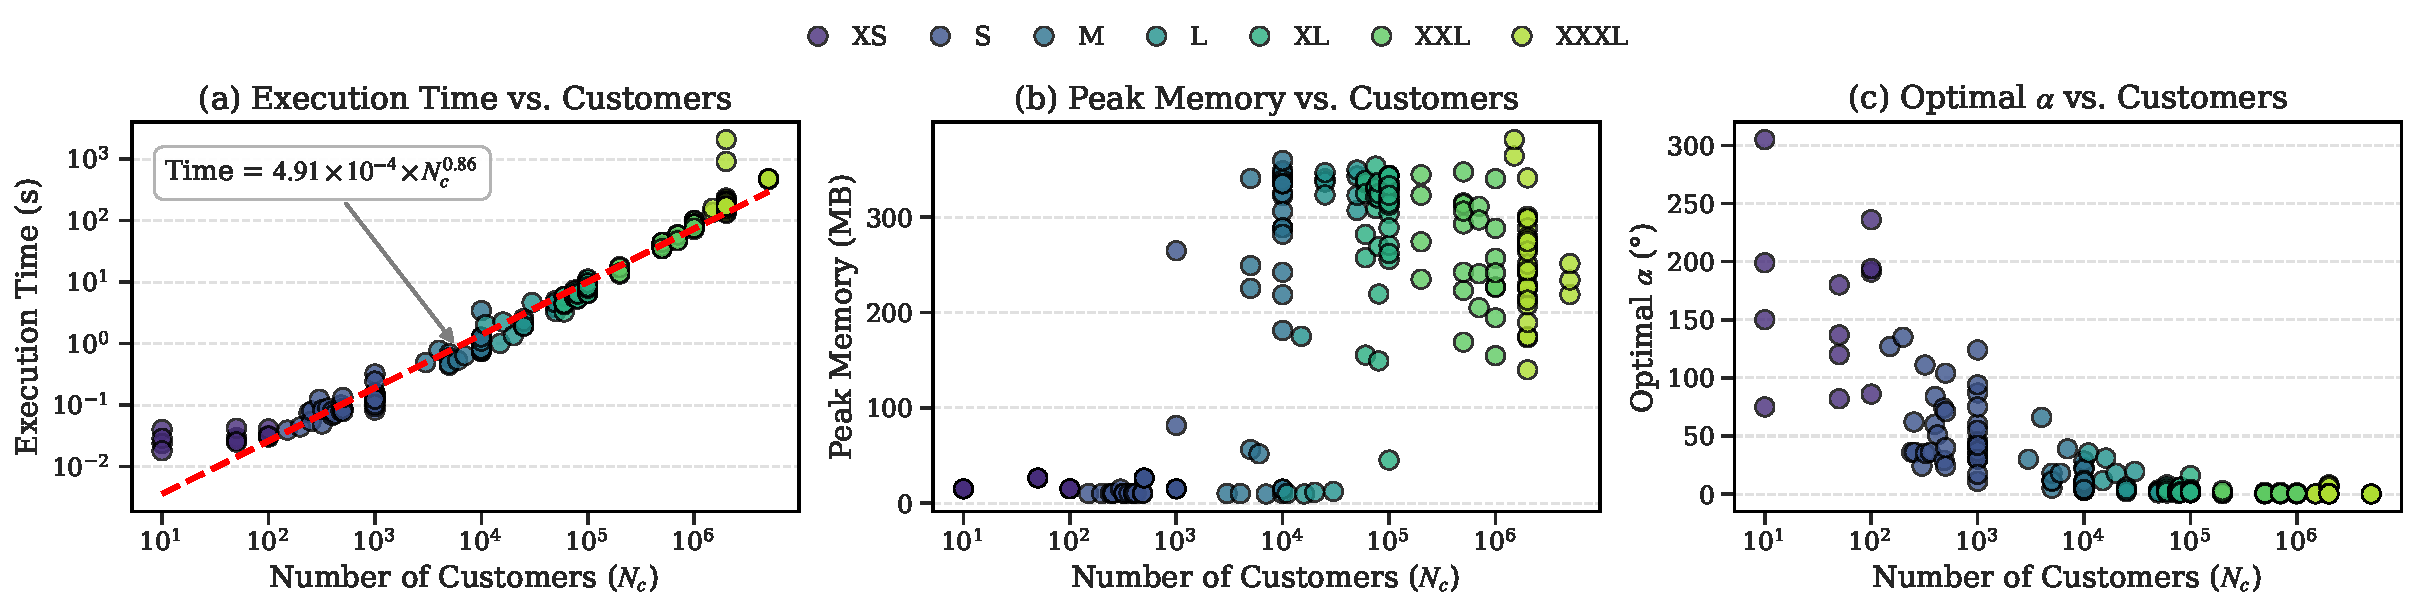
\includegraphics[width=\linewidth]{sections/results/node_Results.pdf}
    \caption{Scalability of BP-MDS: execution time, peak memory and $\alpha$ vs.\ number of customers}
    \label{fig:scalability_grid}
\end{figure*}

To facilitate consistent and scale-aware comparisons, we group datasets into size-based categories based on the number of customers:
XS (1 to 100), S (101 to $10^3$), M ($10^3\!+\!1$ to $10^4$), 
L ($10^4\!+\!1$ to $5\times10^4$), 
XL ($5\times10^4\!+\!1$ to $10^5$), 
XXL ($10^5\!+\!1$ to $10^6$), and 
XXXL ($10^6\!+\!1$ to $10^7$).
Metrics are reported within each category to avoid scale-induced bias in aggregated results. For instance, aggregating results across instances such as \texttt{Golden\_10} (324 nodes) and \texttt{XML\_500000\_3126\_01} (500{,}001 nodes) would otherwise bias the evaluation toward larger instances. All results are averaged over five runs to reduce variance and ensure stability. To reduce RSS overhead from per-thread stack allocation, we set \texttt{OMP\_STACKSIZE}=256KB, which we found sufficient empirically, as BP-MDS uses iterative implementations, heap-allocates its core data structures, and requires minimal stack space. Larger per-thread stacks (4--8 MB) would otherwise increase memory overhead under nested parallelism.

\textbf{Experimental Setup:} All experiments were conducted on a dual-socket Intel Xeon Gold 6248 system with 20 physical cores (40 logical cores) running at 2.50\,GHz, 27.5\,MB of L3 cache, and 192\,GB of RAM. The system runs Red Hat Enterprise Linux 7.6 (64-bit). BP-MDS and all baseline methods were compiled using GCC 9.2.0 with the \texttt{-std=c++17}, \texttt{-O3}, and \texttt{-fopenmp} compiler flags.


\textbf{Input Instances:} We evaluate BP-MDS on 310 CVRP instances\footnote{\label{fn:github}160 synthetic benchmark instances and the optimal BP-MDS partition angle ($\alpha$) for all 310 instances are available in our \href{https://github.com/CodeCraftsmanSandeep/BP-MDS}{GitHub repository}} comprising 130 benchmark instances from CVRPLIB~\cite{Uchoa_CVRPLIB,CVRPLIB}, including X (1--101), Golden (9--20), Antwerp (1--2), Brussels (1--2), Flanders (1--2), Ghent (1--2), Leuven (1--2), CMT5, E-n76-k (10,14), E-n101-k (8,14), F-n135-k7, P-n101-k4, and tai385. To assess scalability, we further include 20 large-scale FILO2 instances~\cite{FILO2} and 160 synthetic (\texttt{XML}-prefixed) instances generated using the CVRPLIB instance generator, covering seven problem scales (XS--XXXL) ranging from $10$ to $5\times10^{6}$ customers. Solution quality ($\mathrm{Gap}=(\mathrm{Cost}-\mathrm{BKS})/\mathrm{BKS}\times 100\%$) is evaluated against the Best-Known Solutions (BKS) reported by CVRPLIB for the 130 benchmark instances and by Accorsi and Vigo~\cite{FILO2} for the 20 FILO2 instances.


Table~\ref{tab:bpmds_per_instance_results} presents per-instance performance, demonstrating scalability to instances with up to 5 million nodes, which are solved within 8 minutes. Table~\ref{tab:avg_metrics_single} summarizes aggregated results across size categories, yielding an overall geometric mean optimality gap of 8.51\%. The 130 CVRPLIB instances achieve a geometric mean gap of 9.67\%\footnote{Reported optimality gaps are computed using the CVRPLIB BKS values available at the time of experimentation.}, while the 20 FILO2 instances achieve a geometric mean gap of 1.27\%. The lower gap on FILO2 is expected, as its Best-Known Solutions (BKS) are taken from the original benchmark, whereas CVRPLIB BKS have been progressively improved through extensive community contributions. To evaluate relative performance, we compare against ParMDS~\cite{Muniasamy_VRP} and the Hybrid Genetic Search (HGS) of Vidal~\cite{vidal2022hybrid}, two state-of-the-art baselines.

\begin{table}[htbp]
\caption{Class-wise aggregated performance of BP-MDS}
\centering
\small
\begin{tabular}{l r r r r r r r r}
\toprule
\multirow{2.5}{*}{\textbf{Size}} & 
\multicolumn{2}{c}{\makecell[c]{\textbf{Avg. Time} \\ \textbf{(s)}}} & 
\multicolumn{2}{c}{\makecell[c]{\textbf{Avg. Mem.} \\ \textbf{(MB)}}} & 
\multicolumn{2}{c}{\makecell[c]{\textbf{Arith. Mean} \\ \textbf{Gap (\%)}}} & 
\multicolumn{2}{c}{\makecell[c]{\textbf{Geo Mean} \\ \textbf{Gap (\%)}}} \\
\cmidrule(lr){2-3} \cmidrule(lr){4-5} \cmidrule(lr){6-7} \cmidrule(lr){8-9}
& \textbf{(a)} & \textbf{(b)} & \textbf{(a)} & \textbf{(b)} & \textbf{(a)} & \textbf{(b)} & \textbf{(a)} & \textbf{(b)} \\
\midrule
XS  & 0.03   & 0.03 & 4.66  & 4.66 & 8.75 & 8.75 & 8.74 & 8.74 \\
S   & 0.09   & 0.09 & 5.35  & 5.35 & 9.77 & 9.77 & 9.70 & 9.70 \\
M   & 1.84   & 1.84 & 17.01 & 17.01 & 9.77 & 9.77 & 9.73 & 9.73 \\
L   & 4.19   & 3.82 & 45.31 & 36.59 & 10.32 & 7.96 & 10.28 & 7.87 \\
XL  & --  & 14.52 & -- & 34.24 & -- & 2.11 & -- & 2.11 \\
XXL & -- & 171.11 & -- & 84.25 & -- & 1.13 & -- & 1.13 \\
\bottomrule
\multicolumn{9}{l}{\footnotesize (a) CVRPLIB 130 instances;  (b) CVRPLIB + FILO2 instances (130+20) instances}
\end{tabular}

\label{tab:avg_metrics_single}
\end{table}

\subsubsection{Comparison Against ParMDS}

We identify a discrepancy in ParMDS: the effective exploration parameter $\rho$ deviates by $\sim\!20\times$ from the reported value. For fairness, we set $\rho$ to the intended value; all reported ParMDS results use this corrected configuration. Fig.~\ref{fig:parMDS_comparison_grid1} compares the performance of BP-MDS against ParMDS. ParMDS exhibits a fundamental scalability limitation: it exhausts system memory beyond $\approx 5 \times 10^{4}$ nodes due to explicit materialization of the complete graph. In contrast, BP-MDS employs an implicit representation, significantly reducing memory usage. 

\begin{figure*}[ht] 
    \centering   
        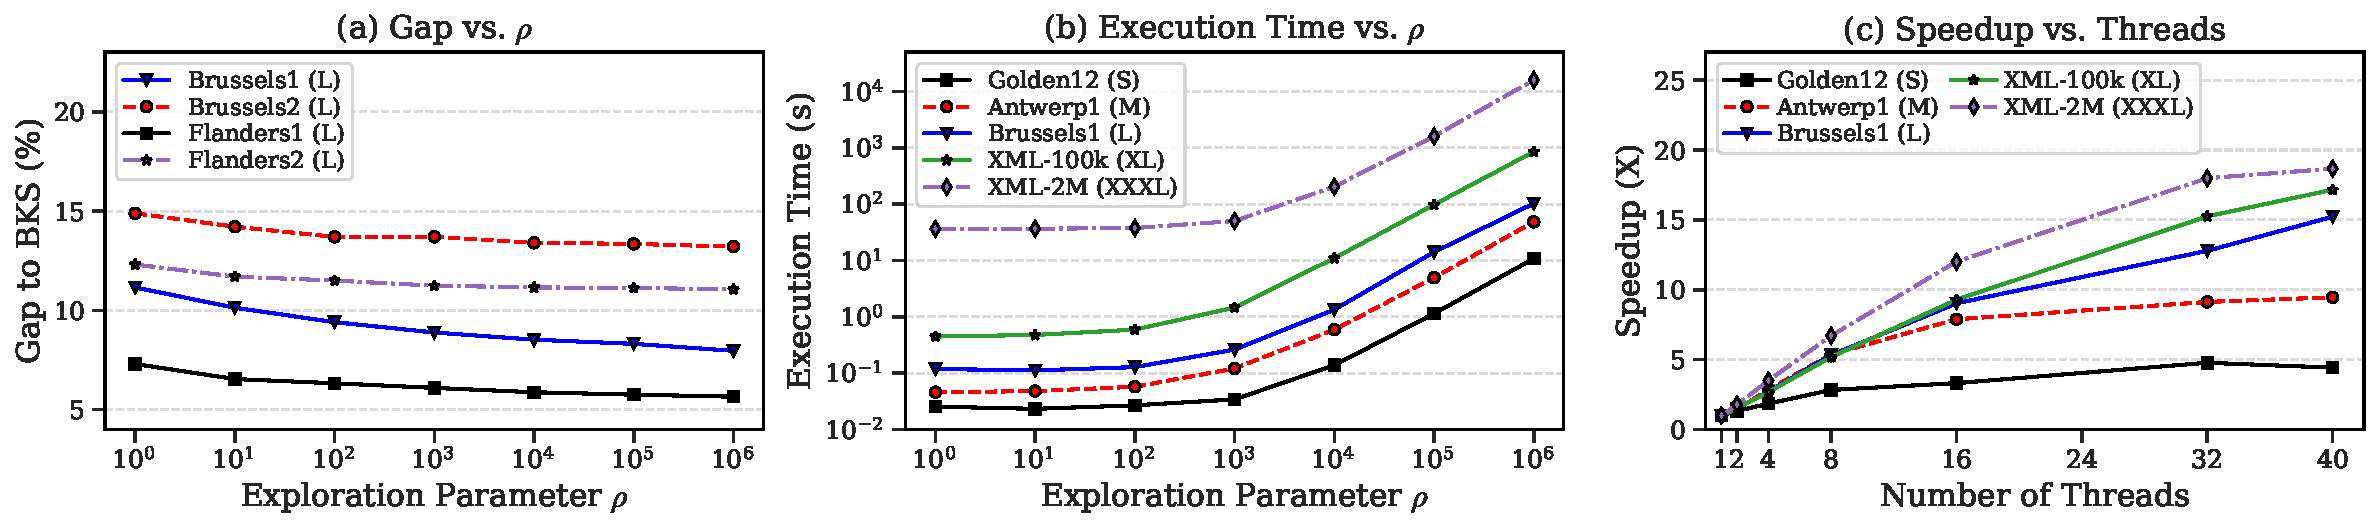
\includegraphics[
    width=\linewidth,
    keepaspectratio
]{sections/results/Parameter_sensitivity.pdf}
    \caption{(a--b) Impact of $\rho$ on solution quality and computational time; (c) Scalability with increasing thread count}
    \label{fig:unified_performance}
\end{figure*}

% ------------------------------------

\begin{figure*}[t]
    \centering
    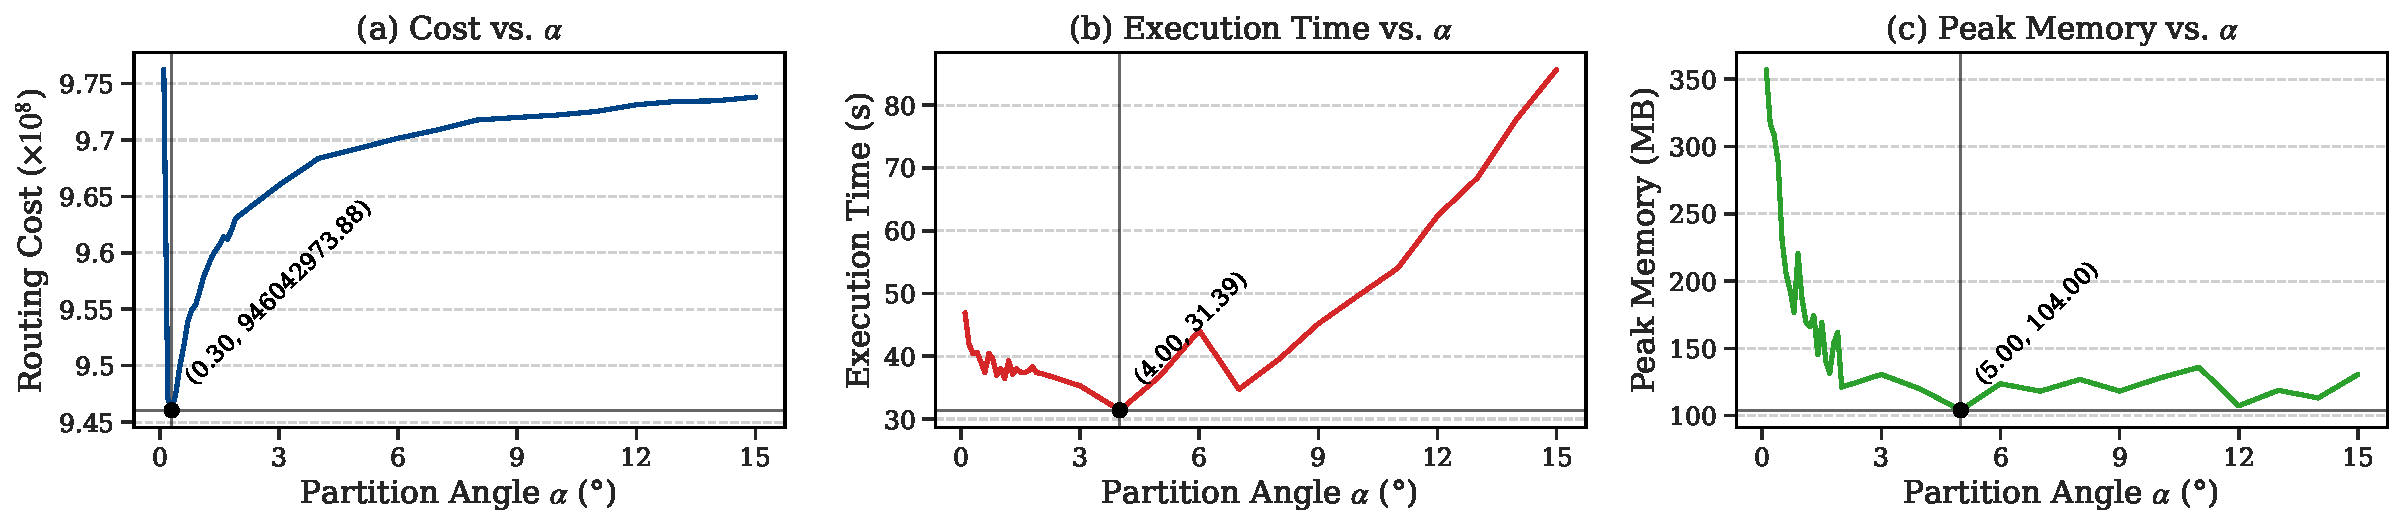
\includegraphics[
    width=\linewidth,
    keepaspectratio
]{sections/results/alpha/XML500000_1173_01_metrics.pdf}
    \caption{Effect of $\alpha$ on cost, execution time, and peak memory}
    \label{fig:alpha_sweep_page1}
\end{figure*}

\textbf{Computational Speedup:} Fig.~\hyperref[fig:parMDS_comparison_grid1]{\ref*{fig:parMDS_comparison_grid1}(a)} shows that BP-MDS achieves consistent execution speedups across all instances, ranging from $5\times$--$10\times$ for S and increasing to $20\times$--$60\times$ for M and L, indicating improved scaling with problem size. The observed speedups stem from massive parallelism and optimized data structures in BP-MDS, absent in ParMDS. 

\textbf{Memory Efficiency:} Fig.~\hyperref[fig:parMDS_comparison_grid1]{\ref*{fig:parMDS_comparison_grid1}(b)} shows that BP-MDS achieves substantial memory savings. While footprints are comparable for small instances, BP-MDS reduces memory usage by $\sim\!100\times$ on M and over $1000\times$ on L instances, enabling scalability to million-node graphs where ParMDS encounters out-of-memory failures. 

\textbf{Solution Quality:} Fig.~\hyperref[fig:parMDS_comparison_grid1]{\ref*{fig:parMDS_comparison_grid1}(c)} shows that BP-MDS consistently reduces the optimality gap across all benchmarks. Gap reductions exceed $10\%$ on S instances and are consistently observed across all evaluated instance sizes, indicating that scalability does not come at the expense of solution quality.

\subsubsection{Comparison Against HGS-CVRP}


\textsc{HGS-CVRP}~\cite{vidal2022hybrid} is a state-of-the-art CVRP solver that delivers high-quality solutions for small instances. Rather than comparing only final solution costs, we perform a time-to-quality analysis. For M and L instances, we measure the time required for HGS-CVRP to match or surpass the solution quality achieved by BP-MDS. For S instances, we report the time to convergence after 20{,}000 iterations. To ensure a fair algorithmic comparison with the single-threaded HGS-CVRP solver, we evaluate BP-MDS under both single-threaded (1T) and 40-threaded (40T) configurations (Table~\ref{tab:bpmds_vs_hgs_time}). For small instances, HGS-CVRP requires between 53 and 108 seconds to converge, whereas BP-MDS executes in under 1 second on a single thread and around $0.1$ seconds using 40 threads. The performance improvement is most pronounced on massive topologies, as observed for \texttt{Flanders1}: BP-MDS generates a high-quality routing plan (5.92\% gap) in just 30.78 seconds with 1 thread and 1.34 seconds with 40 threads, whereas HGS-CVRP takes nearly an hour to achieve the same solution quality. Ultimately, while HGS-CVRP is designed for exhaustive offline optimization to obtain highly optimal solutions, BP-MDS achieves functional routing solutions roughly $90\times$ to $100\times$ faster on a single thread and $350\times$ to $2370\times$ faster using 40 threads, making it well suited for real-time dynamic routing applications across small to massive instances.

\begin{table}[htbp]
\caption{Time-to-quality comparison: BP-MDS vs. HGS-CVRP}
\centering
\small
\setlength{\tabcolsep}{0pt}
\begin{tabular*}{\columnwidth}{@{\extracolsep{\fill}} l c r r r r r r @{}}
\toprule
& & \multicolumn{3}{c}{\textbf{HGS-CVRP}} & \multicolumn{3}{c}{\textbf{BP-MDS (at optimal $\alpha$)}} \\
\cmidrule(lr){3-5} \cmidrule(l){6-8}
\textbf{Instance} & \textbf{Size} & \textbf{Iter.} & \textbf{Time (s)} & \textbf{Gap (\%)} & \textbf{1T (s)} & \textbf{40T (s)} & \textbf{Gap (\%)} \\
\midrule
Golden\_17 & S & 20,000 &   53.80  & 0    &  0.60 & 0.07 & 7.76 \\
Golden\_18 & S & 20,000 &  108.30  & 0    &  0.81 & 0.12 & 4.97 \\
\midrule
Leuven1    & M &      0 &   61.06  & 5.19 &  5.20 & 0.49 & 7.64 \\
Antwerp1   & M &      0 &  185.96  & 5.38 & 10.06 & 0.53 & 7.29 \\
\midrule
Brussels1  & L &     38 & 1562.03  & 8.42 & 23.59 & 1.01 & 8.56 \\
Flanders1  & L &    138 & 3181.58  & 5.62 & 30.78 & 1.34 & 5.92 \\
\bottomrule
\multicolumn{8}{l}{\footnotesize 1T and 40T denote 1 and 40 threads, respectively}
\end{tabular*}
\label{tab:bpmds_vs_hgs_time}
\end{table}

% \begin{table}[htbp]
% \centering
% \setlength{\tabcolsep}{0pt} 
% \begin{tabular*}{\columnwidth}{@{\extracolsep{\fill}} l c r r r r r @{}}
% \toprule
% & & \multicolumn{3}{c}{\textbf{HGS-CVRP}} & \multicolumn{2}{c}{\textbf{BP-MDS}} \\
% \cmidrule(lr){3-5} \cmidrule(l){6-7}
% \textbf{Instance} & \textbf{Size} & \textbf{Iter.} & \textbf{Time (s)} & \textbf{Gap (\%)} & \textbf{Time (s)} & \textbf{Gap (\%)} \\
% \midrule
% Golden\_17 & S & 20,000 &  53.80  & 0 & 0.07 & 4.97  \\
% Golden\_18 & S & 20,000 &  108.30 & 0 & 0.12 & 7.76  \\
% \midrule
% Leuven1    & M &      0 &   61.06 &  5.19 & 0.49 &  7.64 \\
% Antwerp1   & M &      0 &  185.96 &  5.38 & 0.53 &  7.29 \\
% \midrule
% Brussels1  & L &     38 & 1562.03 &  8.42 & 1.01 &  8.56 \\
% Flanders1  & L &    138 & 3181.58 &  5.62 & 1.34 &  5.92 \\
% \bottomrule
% \end{tabular*}
% \caption{Time-to-Quality Comparison: BPMDS vs HGS-CVRP}
% \label{tab:bpmds_vs_hgs_time}
% \end{table}





\subsection{Scalability Study of BP-MDS}
\label{sec:strong_scaling}

\textbf{Execution time and memory scalability:} Figs.~\hyperref[fig:scalability_grid]{\ref*{fig:scalability_grid}(a,b)} show that both execution time and memory consumption increase steadily with problem size. The near-linear growth in execution time demonstrates that BP-MDS scales efficiently to XXXL instances, while the consistent memory trend confirms that bucket partitioning effectively bounds memory overhead.


\textbf{Parallel Scalability:} We evaluate scalability by varying the number of threads from 1 to 40 (Fig.~\hyperref[fig:unified_performance]{\ref*{fig:unified_performance}(c)}). To improve cache locality and avoid thread migration overhead, we enforce thread affinity via \texttt{OMP\_PLACES=cores} and \path{OMP_PROC_BIND=close}. For S and M instances, speedup saturates early and stabilizes well before 40 threads. In these cases, the limited number of angular buckets leads to short MST computations, making OpenMP overhead and thread management dominate useful computation. \REM{As a result, available cores cannot be fully utilized, yielding diminishing returns at higher thread counts.} In contrast, BP-MDS scales efficiently on L--XXXL instances, achieving up to $19\times$ speedup on 40 threads through the high degree of task parallelism provided by thousands of independent angular buckets.

% ------------------------------------
% --- FIGURE: ABLATION STUDY (MINHEAP & DFS PATTERNS) ---
\begin{figure*}[t]
    \centering
    % 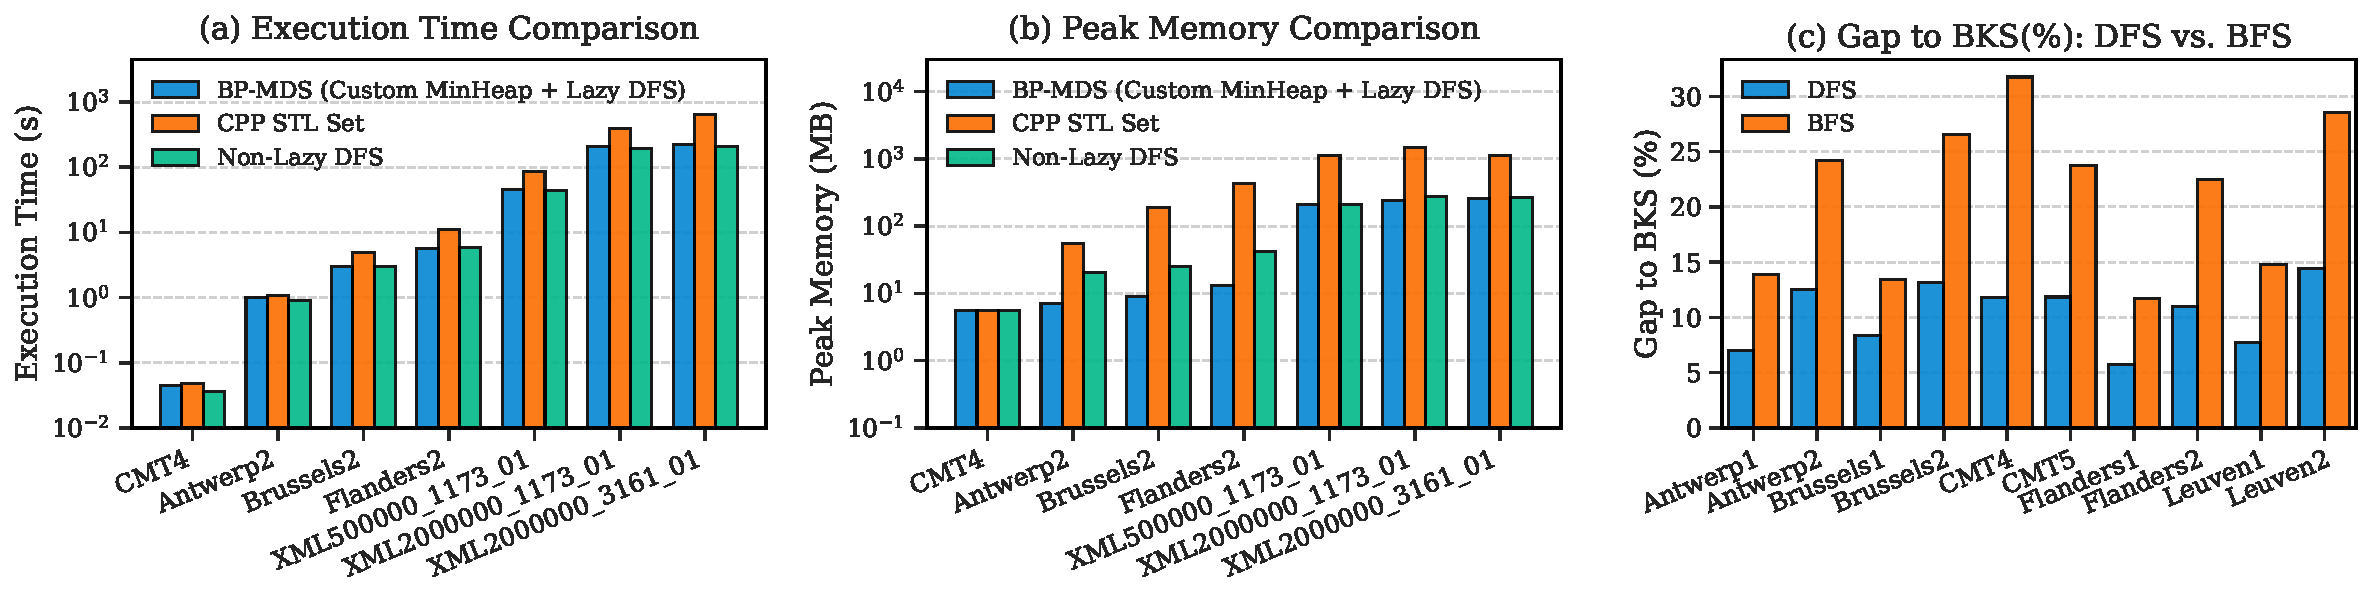
\includegraphics[width=\linewidth]{sections/results/Combined_Ablation_Analysis_Patterns.pdf}

    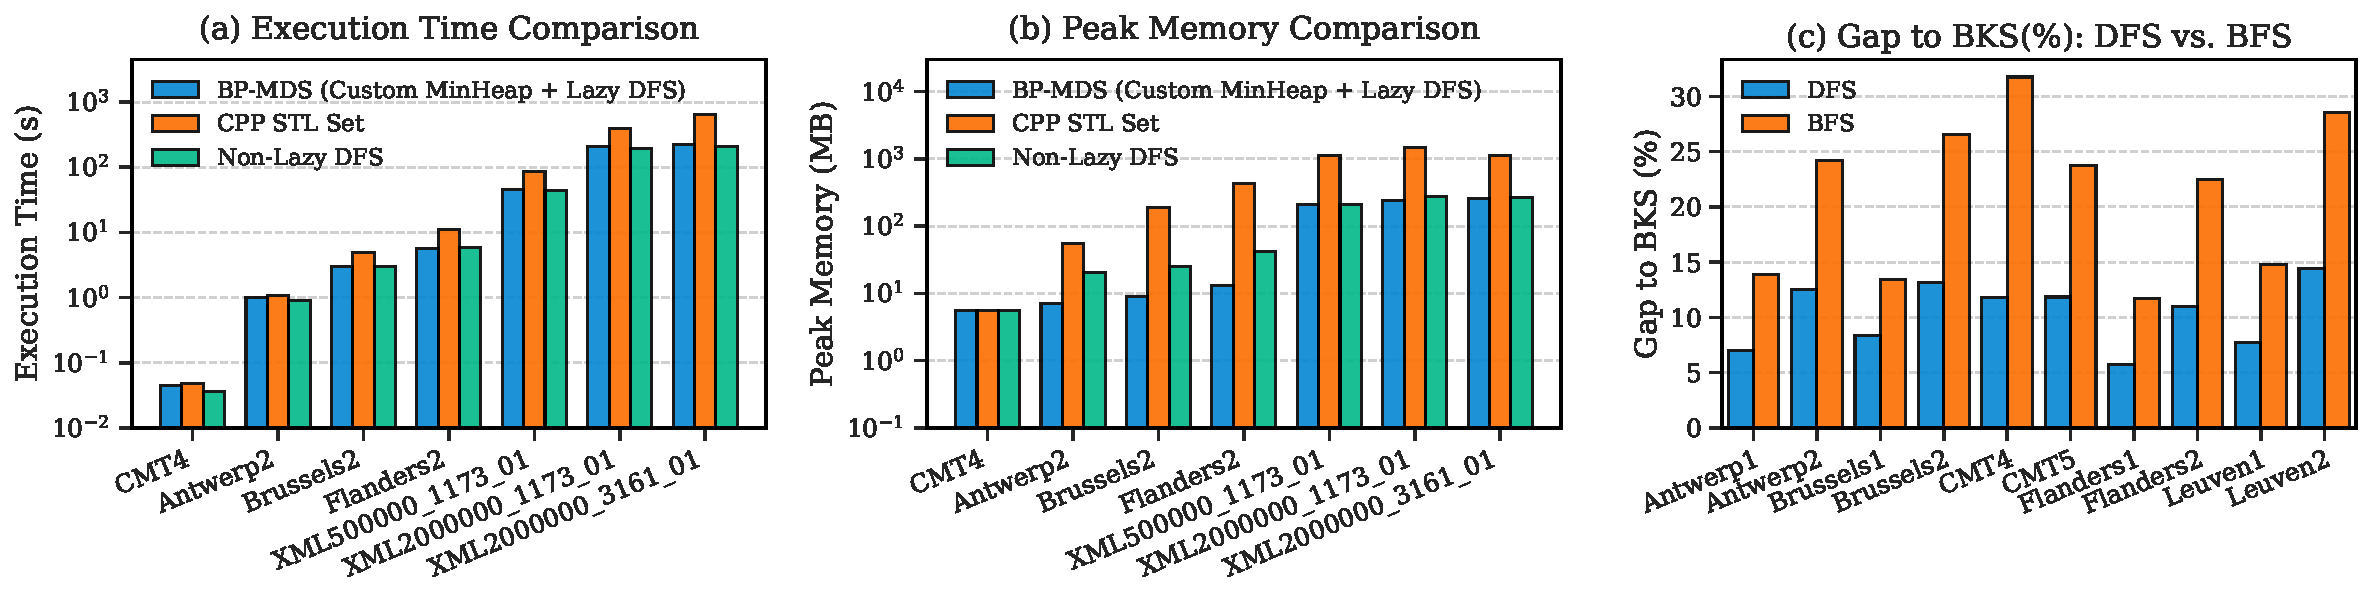
\includegraphics[
    width=\linewidth,
    keepaspectratio
]{sections/results/Combined_Ablation_Analysis_Patterns.pdf}
    \caption{BP-MDS ablation study: Benefits of the custom MinHeap and Lazy DFS, and DFS vs. BFS}
    \label{fig:ablation_analysis}
\end{figure*}



\subsection{Parameter Sensitivity Analysis}
\label{sec:scalability}

\subsubsection{\textbf{Angular Partition Parameter $\alpha$:}} Fig.~\ref{fig:alpha_sweep_page1} illustrates the effect of varying $\alpha$ on solution quality, execution time, and memory consumption. $\alpha$ significantly influences both performance and cost: smaller values of $\alpha$ increase the number of buckets, enabling higher parallelism but also altering solution structure. We select $\alpha$ corresponding to the minimum cost as the empirically best value and refer to it as the optimal $\alpha$ for a given instance size. Fig.~\hyperref[fig:scalability_grid]{\ref*{fig:scalability_grid}(c)} shows that the angular partition parameter $\alpha$ decreases with increasing problem size. This inverse relationship reflects the need for finer bucket partitioning in larger instances, where customer distributions become increasingly structured and exhibit a “flower-like” geometry (Figs.~\ref{fig:BKS_Brussels} and~\ref{fig:2-d-partition}). This enables finer angular buckets to group spatially correlated customers, improving route coherence. 

\textbf{Estimating the Optimal Partition Angle:} The cost-effective $\alpha$ depends on graph scale and spatial density, making manual tuning an additional step in the execution of BP-MDS. To remove this dependency, we propose a simple predictive model that estimates a baseline $\alpha$ directly from graph properties. We use a log-log linear regression with two features: graph dimension ($N$) and total demand-to-capacity ratio ($TD/Q$). Since spatial parameters often follow power-law behavior in routing problems \cite{daganzo1984distance}, we perform regression in logarithmic space, generating a linearized model, a standard approach for modeling multiplicative relationships \cite{hastie2009elements}: $\ln(\alpha) = \ln(k) + c_1 \ln(N) + c_2 \ln\left(\frac{TD}{Q}\right)$. The model is trained on 149 instances ($N > 1000$) with an 80:20 split. In the original scale, it achieves $R^2=0.8376$ (train) and $0.9311$ (test). The learned relation is $\alpha = 949.2975 \cdot N^{-0.1016} \cdot \left(\frac{TD}{Q}\right)^{-0.5509}$, with a test MAE of $3.17^\circ$. \REM{While effective for initialization, incorporating topological features such as route size and depot position may further improve accuracy.}


\subsubsection{\textbf{Exploration Parameter $\rho$}} Increasing $\rho$ reduces the optimality gap (Fig.~\hyperref[fig:unified_performance]{\ref*{fig:unified_performance}(a)}), with the largest gains in the early regime ($\rho \le 10^3$) where randomized DFS quickly identifies high-quality edge combinations. Beyond this, improvements saturate as the local search space within each bucket is exhausted. While low $\rho$ yields higher gaps due to limited exploration, increasing $\rho$ stabilizes solution quality, indicating that BP-MDS avoids poor local optima despite partitioning. However, since the computational effort increases with $\rho$, the execution time also rises accordingly (Fig.~\hyperref[fig:unified_performance]{\ref*{fig:unified_performance}(b)}). Balancing quality and cost, $\rho = 10^4$ emerges as a sweet spot, achieving over $95\%$ of the attainable improvement with modest runtime. \REM{Further increases incur significant overhead with negligible gains.}

% \subsection{Implementation Ablation Study}
\subsection{Ablation Study}
\label{sec:ablation_study} 

\begin{figure*}
    \centering
    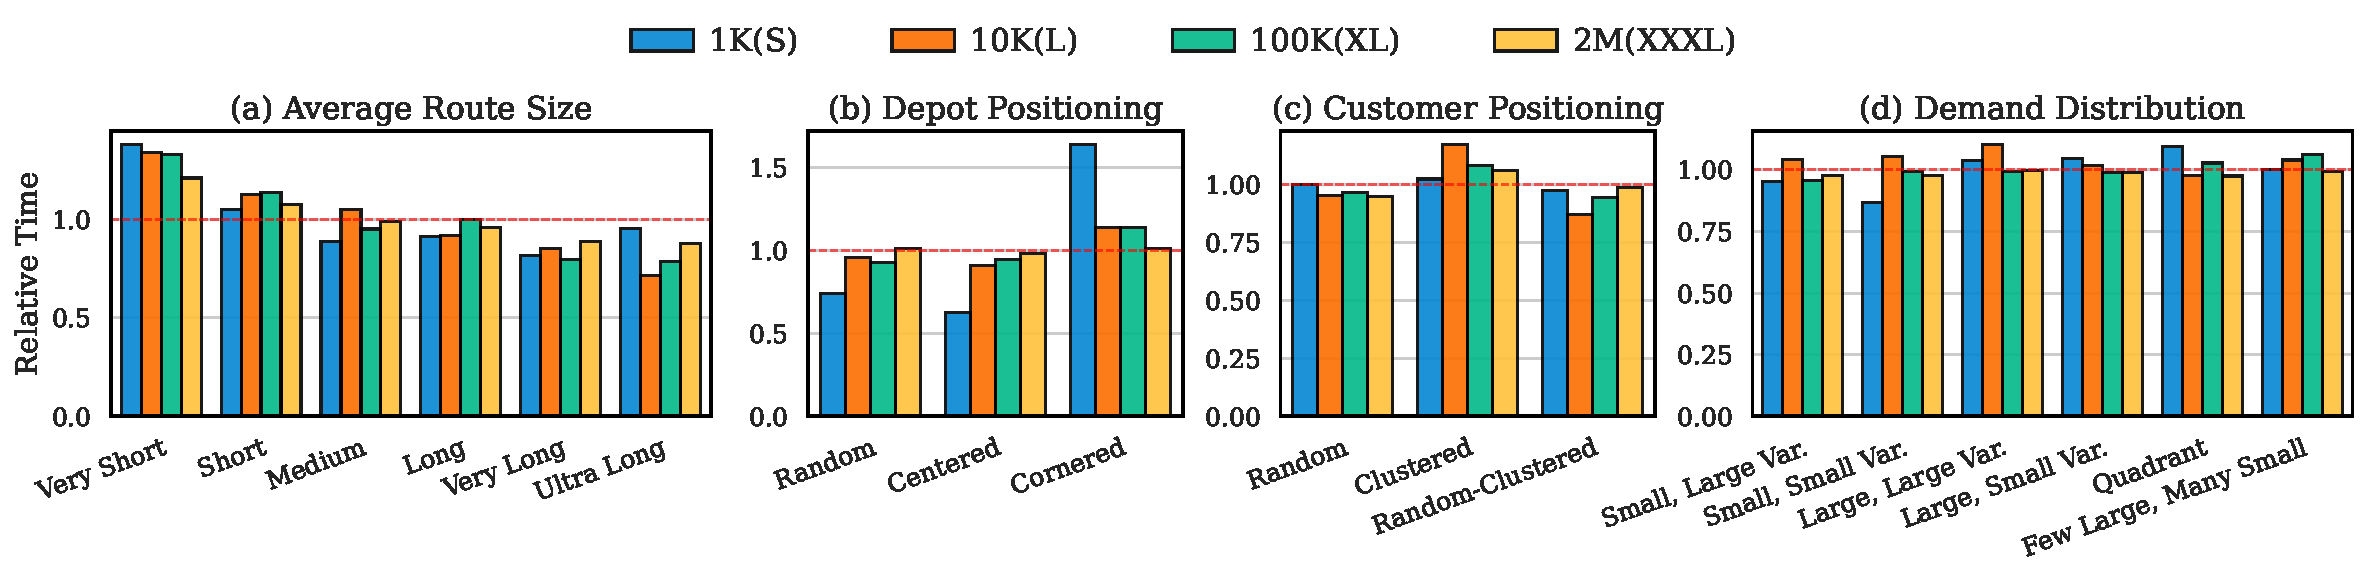
\includegraphics[width=0.94\linewidth]{sections/results/time_plot.pdf}
    
    {\footnotesize Relative time $= T_{g,c}/\bar{T}_g$, where $\bar{T}_g=\frac{1}{|C_g|}\sum_{c\in C_g} T_{g,c}$ is the mean execution time over all instances in category set $C_g$ for graph size $g$}
    \caption{Impact of input characteristics on execution time (at the optimal $\alpha$)}
    \label{fig:characteristics}
\end{figure*}

\begin{figure*}[h]
    \centering
    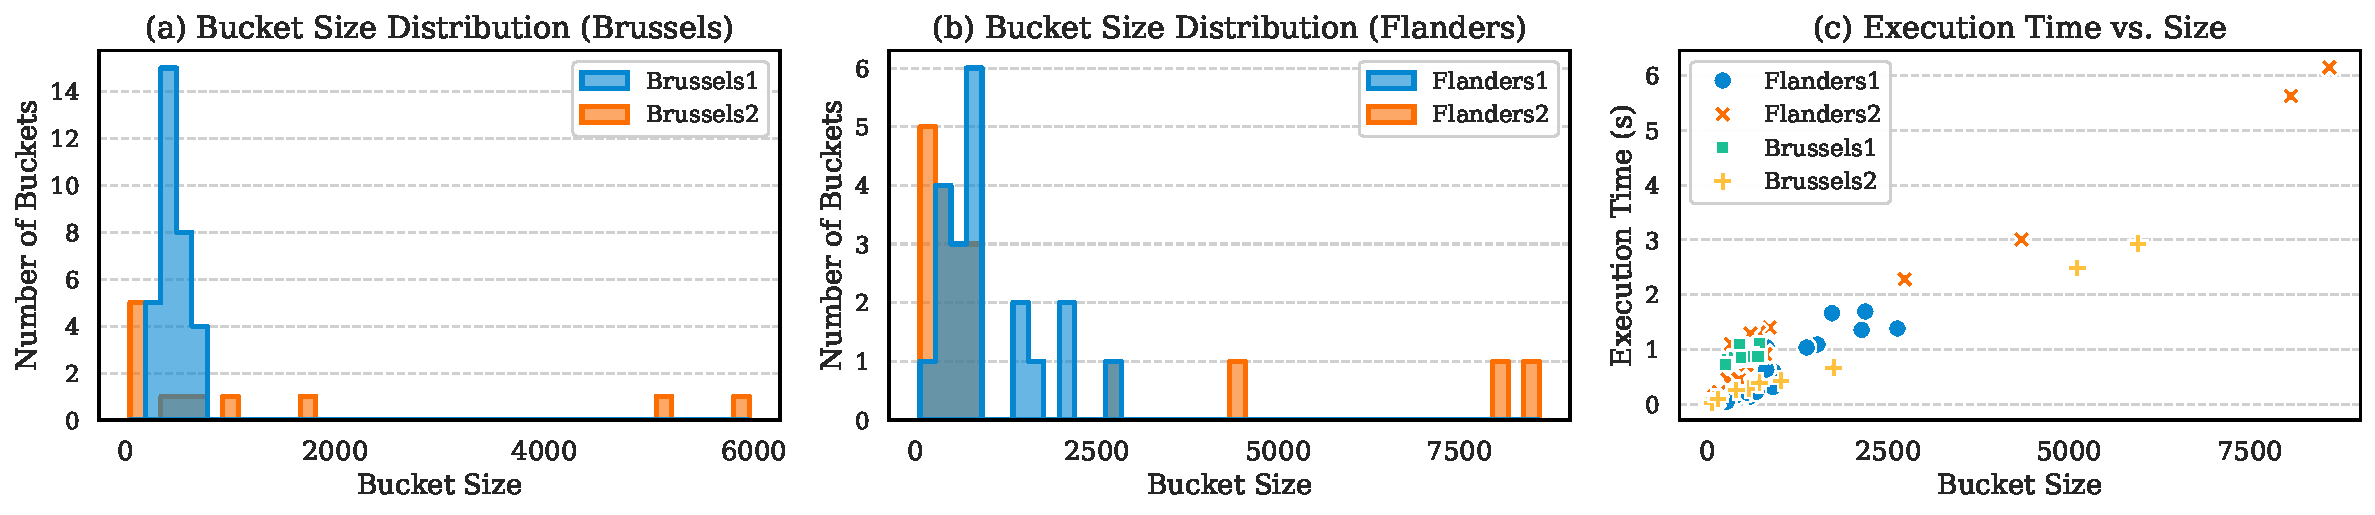
\includegraphics[
    width=\linewidth,
    keepaspectratio
]{sections/results/Bucket_Analysis.pdf}
    \caption{Analysis of centered vs. cornered depots (at the optimal $\alpha$)}
    \label{fig:bucket_analysis}
\end{figure*}

We evaluate three key design choices (Fig.~\ref{fig:ablation_analysis}): a custom MinHeap for Prim's MST, lazy vs. eager DFS, and DFS vs. BFS.


\textbf{Custom MinHeap vs. C++ \texttt{std::set}:} After bucket construction, each thread builds an MST using Prim's algorithm. Our custom \texttt{Min\_Heap} achieves up to a $2.9\times$ speedup (Fig.~\hyperref[fig:ablation_analysis]{\ref*{fig:ablation_analysis}(a)}) by supporting in-place \texttt{DecreaseKey} operations, whereas \texttt{std::set} inserts redundant entries for updated distances, increasing logarithmic overhead. This also substantially reduces memory usage (Fig.~\hyperref[fig:ablation_analysis]{\ref*{fig:ablation_analysis}(b)}): on XXXL instances, \texttt{std::set} uses up to 1.56\,GB due to stale entries, while the custom heap stores one entry per vertex, requiring only 279\,MB.

\textbf{Lazy vs. Eager DFS Traversal:} To generate multiple randomized routes, the MST adjacency list is shuffled before each DFS traversal. \textit{Lazy DFS} copies and shuffles neighbors on demand when a vertex is visited, whereas \textit{Eager DFS} precomputes a deep copy of the entire MST before traversal. Although Eager DFS is marginally faster on large-scale graphs (Fig.~\hyperref[fig:ablation_analysis]{\ref*{fig:ablation_analysis}(a)}), it increases peak memory usage by up to $2.7\times$ (Fig.~\hyperref[fig:ablation_analysis]{\ref*{fig:ablation_analysis}(b)}). In contrast, Lazy DFS bounds per-thread memory consumption while maintaining comparable runtime, making it the preferred strategy for BP-MDS.


\textbf{Why DFS?:} BP-MDS constructs routes by sequentially partitioning the MST traversal order into capacity-feasible routes. By following contiguous root-to-leaf paths, DFS preserves MST connectivity, increasing the likelihood that adjacent vertices in the MST remain within the same route. In contrast, BFS alternates between sibling vertices at the same level, fragmenting MST edges across routes. Consequently, DFS produces lower routing costs than BFS (Fig.~\hyperref[fig:ablation_analysis]{\ref*{fig:ablation_analysis}(c)}). On Flanders (1-2), BFS doubles the optimality gap of DFS.

% Flanders1: BFS\_gap=11.72\%, DFS\_gap=5.78\%, Flanders2: BFS\_gap=22.51\%, DFS\_gap=10.99\%

\subsection{Impact of Input Characteristics}
\label{sec:topology_impact}

% Notes for relative time measurement:
% Times are normalized independently within each graph size category (1K, 10K, 100K, 2M) by dividing by the mean execution time of that scale. The red dashed line ($y = 1.0$) denotes the average computational cost for a graph of that size, highlighting which structural traits inflate or reduce execution overhead.
% For example in subplot (a), for 1K S instances, the mean of all the 6 blue bars is taken and for each bar the time there is divided by this mean. This is done for all S, L, XXL, XXXL seperately

% 

BP-MDS is evaluated on diverse input characteristics (Fig.~\ref{fig:characteristics}) generated using the CVRPLIB input generator. Execution time decreases as the average route size increases, since longer routes reduce the overhead of repeatedly switching between buckets in a parallel setting (Fig.~\hyperref[fig:characteristics]{\ref*{fig:characteristics}(a)}). For the 2M-node instances, increasing the average route size from \emph{Very Short} to \emph{Ultra Long} reduces execution time from 204.04\,s to 151.68\,s. Cornered-depot instances generally require higher execution time than centered or randomly positioned depots (Fig.~\hyperref[fig:characteristics]{\ref*{fig:characteristics}(b)}). This is because cornered depots produce unbalanced bucket sizes, increasing the workload of the largest bucket. On 1K (S) graphs, the cornered depot incurs a $2.47\times$ higher execution time than the centered depot. This behavior is evident in Fig.~\hyperref[fig:bucket_analysis]{\ref*{fig:bucket_analysis}(a,b)}, where \texttt{Brussels2} and \texttt{Flanders2} (cornered depots) exhibit significantly larger buckets than \texttt{Brussels1} and \texttt{Flanders1} (centered depots) (spatial differences are visualized in Fig.~\ref{fig:BKS_Brussels}). Execution time strictly increases with the maximum bucket size (Fig.~\hyperref[fig:bucket_analysis]{\ref*{fig:bucket_analysis}(c)}), confirming that the largest bucket dominates the overall runtime. \REM{In contrast, customer positioning (Fig.~\hyperref[fig:characteristics]{\ref*{fig:characteristics}(c)}) and demand distribution (Fig.~\hyperref[fig:characteristics]{\ref*{fig:characteristics}(d)}) have minimal impact on execution time.}

% {\color{magenta} Demand Distribution among customers. Type 1 assigns a unitary demand of exactly $1$ to all customers, while Types 2 through 5 sample uniformly from fixed intervals: $[1, 10]$ (small, large variance), $[5, 10]$ (small, small variance), $[1, 100]$ (large, large variance), and $[50, 100]$ (large, small variance). For Quadrant, Customers in "even quadrants" (bottom-left where $x,y < 5000$, or top-right where $x,y \ge 5000$) get large demands sampled uniformly from $[51, 100]$.  Customers in the other two quadrants get smaller demands sampled from $[1, 50]$. A calculated proportion of customers ($\frac{n}{r} \times 1.5$, where $r$ is target route size) receive large demands uniformly sampled from $[50, 100]$.  All remaining customers receive small demands sampled from $[1, 10]$. 
% Average Route Size (avgRouteSize) controls the expected number of customers served per vehicle by uniformly sampling a target continuous value $r$(route size) from one of six category intervals: Very short $[3, 5]$, Short $[5, 8]$, Medium $[8, 12]$, Long $[12, 16]$, Very long $[16, 25]$, and Ultra long $[25, 50]$. 
% Depot Positioning establishes the starting hub location on a $10{,}000 \times 10{,}000$ 2D Euclidean grid according to three simple placement strategies. Type 1 (Random) places the depot uniformly at random anywhere within the $[0, 10000]$ coordinate range. Type 2 (Centered) fixes the depot exactly at the midpoint of the grid at coordinates $(5000, 5000)$. Type 3 (Cornered) fixes the depot at the bottom-left origin point $(0, 0)$.  
% Customer Positioning (custPos) distributes the $n$ customer coordinates across the same $10{,}000 \times 10{,}000$ Euclidean grid using three distinct spatial patterns. Type 1 (Random) generates all customer coordinates uniformly at random across the entire grid. Type 2 (Clustered) generates between 2 to 6 random seed centers and places customers around them using an Accept-Reject method. Type 3 (Random-Clustered) is a 50/50 hybrid model where half of the customers ($n/2$) are generated uniformly at random and the remaining half are generated around seed centers using the exponential decay clustering method.}

%  The below two paras are related to: Impact of graph topology on alpha. This is removed because of lack of space. 
% Fig.~\hyperref[fig:characteristics]{\ref*{fig:characteristics}(a)} shows that $\alpha$ increases with average route size, since larger routes require a wider angular sweep to accumulate sufficient customers for feasible vehicle capacity. Fig.~\hyperref[fig:characteristics]{\ref*{fig:characteristics}(b)} shows that a centered depot yields higher $\alpha$ than cornered or random placements, as central positioning spreads customers over a full $360^\circ$ range, requiring wider partitions to capture enough nodes per bucket. Fig.~\hyperref[fig:characteristics]{\ref*{fig:characteristics}(c)} shows that clustered customer distributions also increase $\alpha$, as overly narrow partitions fragment spatial clusters and break short-distance route coherence.

% Across all cases, graph scale dominates these effects: as the number of nodes increases, sensitivity to topology diminishes and $\alpha$ consistently converges to smaller angular values. This is because higher node density reduces the need for wide partitions, allowing efficient routing within narrow angular regions. Overall, BP-MDS adapts to topology at small scales but becomes scale-dominated, where dense graphs enforce uniform, highly fine-grained partitioning without loss of routing quality.




\section{Conclusion and Future Work}

We presented BP-MDS, a parallel divide-and-conquer framework for million-scale CVRP. Experiments demonstrate that BP-MDS achieves an 8.51\% geometric mean optimality gap while delivering substantial speedups over state-of-the-art CPU-based methods, enabling efficient solution of million-customer instances. It provides an effective trade-off between solution quality and execution time. BP-MDS incorporates 2-opt for intra-route refinement and improves route quality through randomized intra-bucket exploration. It does not optimize customer assignments across routes or buckets. Scalable inter-route and inter-bucket optimization is left as future work. Other directions include establishing theoretical bounds on solution quality, multiple MSTs per bucket, adaptive partitioning, and scaling to billion-scale inputs on CPU--GPU systems.



% \begin{acks}
% The last author was partially supported by the
% \grantsponsor{fedex-centre}{FedEx Centre}{}
% under Grant No.\
% \grantnum{fedex-centre}{SB24250339CSFEDX008103}.
% \end{acks}

% \begin{acks}
% The last author is partially supported by the FedEx Centre research grant SB24250339CSFEDX008103.
% \end{acks}

% {\small
% \ \\\noindent{{\bf Acknowledgments.} The last author is partially supported by the FedEx Centre research grant SB24250339CSFEDX008103.}
% }


\bibliographystyle{ACM-Reference-Format}
\bibliography{references}

\end{document}
